% Options for packages loaded elsewhere
\PassOptionsToPackage{unicode}{hyperref}
\PassOptionsToPackage{hyphens}{url}
\documentclass[
  10pt,
]{article}
\usepackage{xcolor}
\usepackage[margin=1in]{geometry}
\usepackage{amsmath,amssymb}
\setcounter{secnumdepth}{5}
\usepackage{iftex}
\ifPDFTeX
  \usepackage[T1]{fontenc}
  \usepackage[utf8]{inputenc}
  \usepackage{textcomp} % provide euro and other symbols
\else % if luatex or xetex
  \usepackage{unicode-math} % this also loads fontspec
  \defaultfontfeatures{Scale=MatchLowercase}
  \defaultfontfeatures[\rmfamily]{Ligatures=TeX,Scale=1}
\fi
\usepackage{lmodern}
\ifPDFTeX\else
  % xetex/luatex font selection
\fi
% Use upquote if available, for straight quotes in verbatim environments
\IfFileExists{upquote.sty}{\usepackage{upquote}}{}
\IfFileExists{microtype.sty}{% use microtype if available
  \usepackage[]{microtype}
  \UseMicrotypeSet[protrusion]{basicmath} % disable protrusion for tt fonts
}{}
\makeatletter
\@ifundefined{KOMAClassName}{% if non-KOMA class
  \IfFileExists{parskip.sty}{%
    \usepackage{parskip}
  }{% else
    \setlength{\parindent}{0pt}
    \setlength{\parskip}{6pt plus 2pt minus 1pt}}
}{% if KOMA class
  \KOMAoptions{parskip=half}}
\makeatother
\usepackage{color}
\usepackage{fancyvrb}
\newcommand{\VerbBar}{|}
\newcommand{\VERB}{\Verb[commandchars=\\\{\}]}
\DefineVerbatimEnvironment{Highlighting}{Verbatim}{commandchars=\\\{\}}
% Add ',fontsize=\small' for more characters per line
\usepackage{framed}
\definecolor{shadecolor}{RGB}{248,248,248}
\newenvironment{Shaded}{\begin{snugshade}}{\end{snugshade}}
\newcommand{\AlertTok}[1]{\textcolor[rgb]{0.94,0.16,0.16}{#1}}
\newcommand{\AnnotationTok}[1]{\textcolor[rgb]{0.56,0.35,0.01}{\textbf{\textit{#1}}}}
\newcommand{\AttributeTok}[1]{\textcolor[rgb]{0.13,0.29,0.53}{#1}}
\newcommand{\BaseNTok}[1]{\textcolor[rgb]{0.00,0.00,0.81}{#1}}
\newcommand{\BuiltInTok}[1]{#1}
\newcommand{\CharTok}[1]{\textcolor[rgb]{0.31,0.60,0.02}{#1}}
\newcommand{\CommentTok}[1]{\textcolor[rgb]{0.56,0.35,0.01}{\textit{#1}}}
\newcommand{\CommentVarTok}[1]{\textcolor[rgb]{0.56,0.35,0.01}{\textbf{\textit{#1}}}}
\newcommand{\ConstantTok}[1]{\textcolor[rgb]{0.56,0.35,0.01}{#1}}
\newcommand{\ControlFlowTok}[1]{\textcolor[rgb]{0.13,0.29,0.53}{\textbf{#1}}}
\newcommand{\DataTypeTok}[1]{\textcolor[rgb]{0.13,0.29,0.53}{#1}}
\newcommand{\DecValTok}[1]{\textcolor[rgb]{0.00,0.00,0.81}{#1}}
\newcommand{\DocumentationTok}[1]{\textcolor[rgb]{0.56,0.35,0.01}{\textbf{\textit{#1}}}}
\newcommand{\ErrorTok}[1]{\textcolor[rgb]{0.64,0.00,0.00}{\textbf{#1}}}
\newcommand{\ExtensionTok}[1]{#1}
\newcommand{\FloatTok}[1]{\textcolor[rgb]{0.00,0.00,0.81}{#1}}
\newcommand{\FunctionTok}[1]{\textcolor[rgb]{0.13,0.29,0.53}{\textbf{#1}}}
\newcommand{\ImportTok}[1]{#1}
\newcommand{\InformationTok}[1]{\textcolor[rgb]{0.56,0.35,0.01}{\textbf{\textit{#1}}}}
\newcommand{\KeywordTok}[1]{\textcolor[rgb]{0.13,0.29,0.53}{\textbf{#1}}}
\newcommand{\NormalTok}[1]{#1}
\newcommand{\OperatorTok}[1]{\textcolor[rgb]{0.81,0.36,0.00}{\textbf{#1}}}
\newcommand{\OtherTok}[1]{\textcolor[rgb]{0.56,0.35,0.01}{#1}}
\newcommand{\PreprocessorTok}[1]{\textcolor[rgb]{0.56,0.35,0.01}{\textit{#1}}}
\newcommand{\RegionMarkerTok}[1]{#1}
\newcommand{\SpecialCharTok}[1]{\textcolor[rgb]{0.81,0.36,0.00}{\textbf{#1}}}
\newcommand{\SpecialStringTok}[1]{\textcolor[rgb]{0.31,0.60,0.02}{#1}}
\newcommand{\StringTok}[1]{\textcolor[rgb]{0.31,0.60,0.02}{#1}}
\newcommand{\VariableTok}[1]{\textcolor[rgb]{0.00,0.00,0.00}{#1}}
\newcommand{\VerbatimStringTok}[1]{\textcolor[rgb]{0.31,0.60,0.02}{#1}}
\newcommand{\WarningTok}[1]{\textcolor[rgb]{0.56,0.35,0.01}{\textbf{\textit{#1}}}}
\usepackage{graphicx}
\makeatletter
\newsavebox\pandoc@box
\newcommand*\pandocbounded[1]{% scales image to fit in text height/width
  \sbox\pandoc@box{#1}%
  \Gscale@div\@tempa{\textheight}{\dimexpr\ht\pandoc@box+\dp\pandoc@box\relax}%
  \Gscale@div\@tempb{\linewidth}{\wd\pandoc@box}%
  \ifdim\@tempb\p@<\@tempa\p@\let\@tempa\@tempb\fi% select the smaller of both
  \ifdim\@tempa\p@<\p@\scalebox{\@tempa}{\usebox\pandoc@box}%
  \else\usebox{\pandoc@box}%
  \fi%
}
% Set default figure placement to htbp
\def\fps@figure{htbp}
\makeatother
\setlength{\emergencystretch}{3em} % prevent overfull lines
\providecommand{\tightlist}{%
  \setlength{\itemsep}{0pt}\setlength{\parskip}{0pt}}
\usepackage{titling}

\pretitle{%
  \begin{center}
  \LARGE
    \includegraphics[width=1cm]{/export/scratch2/Rplus/Rlogo.png}
}
\posttitle{\end{center}}

\usepackage{array, lipsum, bibentry,fancyhdr,hyperref,color,amsmath}
\pagestyle{fancy}
\fancyhf{}
\lhead{P.BADY}
\chead{}
\cfoot{\thepage}
\rhead{Tumor size progression in LGG population}
\renewcommand{\headrulewidth}{1pt}
\renewcommand{\footrulewidth}{1pt}
\usepackage{bookmark}
\IfFileExists{xurl.sty}{\usepackage{xurl}}{} % add URL line breaks if available
\urlstyle{same}
\hypersetup{
  pdftitle={Working Notes: Data Analysis with R{,} Python and Rcpp (version 0.999)},
  pdfauthor={P.BADY},
  hidelinks,
  pdfcreator={LaTeX via pandoc}}

\title{\textbf{Working Notes:} Data Analysis with R, Python and Rcpp
(version 0.999)}
\author{\textbf{P.BADY}}
\date{Date: 2026-07-21}

\begin{document}
\maketitle

{
\setcounter{tocdepth}{5}
\tableofcontents
}
\newpage

\begin{itemize}
\tightlist
\item
  \textbf{Contributor:} P.BADY
\item
  \textbf{Date:} `2024-02-26'
\item
  \textbf{Revision:} Tue Jul 21 15:01:21 2026
\item
  \textbf{Abstract:}
\end{itemize}

\rule{1\linewidth}{0.5pt}

\begin{verbatim}
The document investigates the evolution/progression of the tumor size (volume) 
before the the first TMZ treatment in Low grade Glioma (codeleted and 
non-codeleted IDH mutant patients) from Montpellier cohort. Several methods 
were used to estimate the estimation of the growth rate such as linear mixed 
model, non-linear models with bayesian estimation.
\end{verbatim}

\rule{1\linewidth}{0.5pt}

\begin{itemize}
\tightlist
\item
  \textbf{Keywords:} python, C/C++, pandas, numpy, R, dudi,
  multifactorial analyses
\end{itemize}

\rule{1\linewidth}{0.5pt}

\begin{verbatim}
License: GPL version 2 or newer
Copyright (C) 2001-2023  Pierre Bady

This program is free software/document; you can redistribute it and/or
modify it under the terms of the GNU General Public License
as published by the Free Software Foundation; either version 2
of the License, or (at your option) any later version.

This program/document is distributed in the hope that it will be useful,
but WITHOUT ANY WARRANTY; without even the implied warranty of
MERCHANTABILITY or FITNESS FOR A PARTICULAR PURPOSE.  See the
GNU General Public License for more details.
\end{verbatim}

\rule{1\linewidth}{0.5pt}

\newpage

\definecolor{Soutput}{rgb}{0,0,0.56}
\definecolor{Sinput}{rgb}{0.56,0,0}

\section{Motivations}\label{motivations}

The objective of this document is to propose an implementation of data
analysis methods based on duality diagram in python and to develop and
expand my skill in python. The document contains information related to
the use of Rcpp (R and C++).

\section{first test PCA based on R package
ade4}\label{first-test-pca-based-on-r-package-ade4}

\subsection{Example from the R package
ade4}\label{example-from-the-r-package-ade4}

\begin{Shaded}
\begin{Highlighting}[]
\NormalTok{library(ade4)}
\NormalTok{data(deug)}
\NormalTok{pca1 \textless{}{-} dudi.pca(deug$tab, center = deug$cent, scale = FALSE, scan = FALSE)}
\NormalTok{pca2 \textless{}{-} dudi.pca(deug$tab, center = TRUE, scale = TRUE, scan = FALSE)}
\end{Highlighting}
\end{Shaded}

The script can be directly usd in Rstudio and R via the R package
reticulate (\url{https://rstudio.github.io/reticulate/}).

\begin{Shaded}
\begin{Highlighting}[]
\NormalTok{write.csv(deug$tab,file="data/deugtab.csv")}
\end{Highlighting}
\end{Shaded}

\subsection{Data importation}\label{data-importation}

see for example:
\url{https://www.kaggle.com/code/arnopub/pandas-pr-sentation-des-dataframe}

\begin{Shaded}
\begin{Highlighting}[]
\NormalTok{import numpy as np }
\NormalTok{import pandas as pd}
\NormalTok{deugtab = pd.read\_csv(\textquotesingle{}data/deugtab.csv\textquotesingle{})}
\NormalTok{deugtab}
\end{Highlighting}
\end{Shaded}

\begin{verbatim}
##      Unnamed: 0  Algebra  Analysis  Proba  ...  Option1  Option2  English  Sport
## 0             1       40      26.0     26  ...       17     24.0     19.0   11.5
## 1             2       37      34.5     37  ...       24     22.0     26.0   11.5
## 2             3       37      41.0     29  ...       24     27.0     19.6   11.5
## 3             4       63      37.5     57  ...       23     23.0     21.0   14.0
## 4             5       55      31.5     34  ...       19     24.0     24.0   11.5
## ..          ...      ...       ...    ...  ...      ...      ...      ...    ...
## 99          100       60      41.0     18  ...       20     24.0     17.2    0.0
## 100         101       48      44.0     22  ...       22     28.0     19.6    0.0
## 101         102       44      45.0     42  ...       27     22.0     18.4   15.0
## 102         103       47      32.0     26  ...       23     28.0     19.0   11.5
## 103         104       44      32.0     42  ...       28     27.5     23.0   11.5
## 
## [104 rows x 10 columns]
\end{verbatim}

\begin{Shaded}
\begin{Highlighting}[]
\NormalTok{del deugtab[\textquotesingle{}Unnamed: 0\textquotesingle{}]}
\NormalTok{deugtab}
\end{Highlighting}
\end{Shaded}

\begin{verbatim}
##      Algebra  Analysis  Proba  Informatic  ...  Option1  Option2  English  Sport
## 0         40      26.0     26        26.0  ...       17     24.0     19.0   11.5
## 1         37      34.5     37        32.0  ...       24     22.0     26.0   11.5
## 2         37      41.0     29        34.5  ...       24     27.0     19.6   11.5
## 3         63      37.5     57        35.5  ...       23     23.0     21.0   14.0
## 4         55      31.5     34        36.0  ...       19     24.0     24.0   11.5
## ..       ...       ...    ...         ...  ...      ...      ...      ...    ...
## 99        60      41.0     18        30.0  ...       20     24.0     17.2    0.0
## 100       48      44.0     22        30.0  ...       22     28.0     19.6    0.0
## 101       44      45.0     42        35.0  ...       27     22.0     18.4   15.0
## 102       47      32.0     26        21.0  ...       23     28.0     19.0   11.5
## 103       44      32.0     42        26.5  ...       28     27.5     23.0   11.5
## 
## [104 rows x 9 columns]
\end{verbatim}

\section{PCA from scratch in python}\label{pca-from-scratch-in-python}

PCA from scratch
(\url{https://towardsdatascience.com/principal-component-analysis-from-scratch-in-numpy-61843da1f967})

\begin{Shaded}
\begin{Highlighting}[]
\NormalTok{\# centering = TRUE}
\NormalTok{X= deugtab {-} deugtab.mean()}
\NormalTok{\# Normalize}
\NormalTok{Z = X / X.std(ddof=0)}
\NormalTok{print(\textquotesingle{}MEAN:\textquotesingle{})}
\end{Highlighting}
\end{Shaded}

\begin{verbatim}
## MEAN:
\end{verbatim}

\begin{Shaded}
\begin{Highlighting}[]
\NormalTok{print(Z.mean())}
\end{Highlighting}
\end{Shaded}

\begin{verbatim}
## Algebra      -9.394195e-17
## Analysis      3.928481e-16
## Proba        -1.003471e-16
## Informatic   -1.579933e-16
## Economy       4.782499e-16
## Option1      -1.281027e-17
## Option2       1.814788e-16
## English      -9.137990e-16
## Sport         1.665335e-16
## dtype: float64
\end{verbatim}

\begin{Shaded}
\begin{Highlighting}[]
\NormalTok{print(\textquotesingle{}{-}{-}{-}\textquotesingle{}*15)}
\end{Highlighting}
\end{Shaded}

\begin{verbatim}
## ---------------------------------------------
\end{verbatim}

\begin{Shaded}
\begin{Highlighting}[]
\NormalTok{print(\textquotesingle{}STD:\textquotesingle{})}
\end{Highlighting}
\end{Shaded}

\begin{verbatim}
## STD:
\end{verbatim}

\begin{Shaded}
\begin{Highlighting}[]
\NormalTok{print(Z.std(ddof=0))}
\end{Highlighting}
\end{Shaded}

\begin{verbatim}
## Algebra       1.0
## Analysis      1.0
## Proba         1.0
## Informatic    1.0
## Economy       1.0
## Option1       1.0
## Option2       1.0
## English       1.0
## Sport         1.0
## dtype: float64
\end{verbatim}

diagonalisation and eigenvectors

\begin{Shaded}
\begin{Highlighting}[]
\NormalTok{import numpy as np}
\NormalTok{len(Z)}
\end{Highlighting}
\end{Shaded}

\begin{verbatim}
## 104
\end{verbatim}

\begin{Shaded}
\begin{Highlighting}[]
\NormalTok{ZZ = np.dot(Z.T, Z)/len(Z)}
\NormalTok{eigenvalues, eigenvectors = np.linalg.eig(ZZ)}
\NormalTok{D = np.diag(eigenvalues)}
\NormalTok{P = eigenvectors}
\NormalTok{Z\_new = np.dot(Z, P)}
\end{Highlighting}
\end{Shaded}

valeur propres non ordonnées !!!!

Calculate the proportion of variance explained by each feature

\begin{Shaded}
\begin{Highlighting}[]
\NormalTok{sum\_eigenvalues = np.sum(eigenvalues)}
\NormalTok{sum\_eigenvalues}
\end{Highlighting}
\end{Shaded}

\begin{verbatim}
## 9.000000000000002
\end{verbatim}

\begin{Shaded}
\begin{Highlighting}[]
\NormalTok{prop\_var = [i/sum\_eigenvalues for i in eigenvalues]}
\end{Highlighting}
\end{Shaded}

Calculate the cumulative variance

\begin{Shaded}
\begin{Highlighting}[]
\NormalTok{cum\_var = [np.sum(prop\_var[:i+1]) for i in range(len(prop\_var))]}
\end{Highlighting}
\end{Shaded}

Plot scree plot from PCA

\begin{Shaded}
\begin{Highlighting}[]
\NormalTok{import matplotlib.pyplot as plt}
\NormalTok{x\_labels = [\textquotesingle{}PC\{\}\textquotesingle{}.format(i+1) for i in range(len(prop\_var))]}
\NormalTok{plt.plot(x\_labels, prop\_var, marker=\textquotesingle{}o\textquotesingle{}, markersize=6, color=\textquotesingle{}skyblue\textquotesingle{}, }
\NormalTok{  linewidth=2, label=\textquotesingle{}Proportion of variance\textquotesingle{})}
\NormalTok{plt.plot(x\_labels, cum\_var, marker=\textquotesingle{}o\textquotesingle{}, color=\textquotesingle{}orange\textquotesingle{}, linewidth=2, }
\NormalTok{  label="Cumulative variance")}
\NormalTok{plt.legend()}
\NormalTok{plt.title(\textquotesingle{}Scree plot\textquotesingle{})}
\NormalTok{plt.xlabel(\textquotesingle{}Principal components\textquotesingle{})}
\NormalTok{plt.ylabel(\textquotesingle{}Proportion of variance\textquotesingle{})}
\NormalTok{plt.show()}
\end{Highlighting}
\end{Shaded}

\pandocbounded{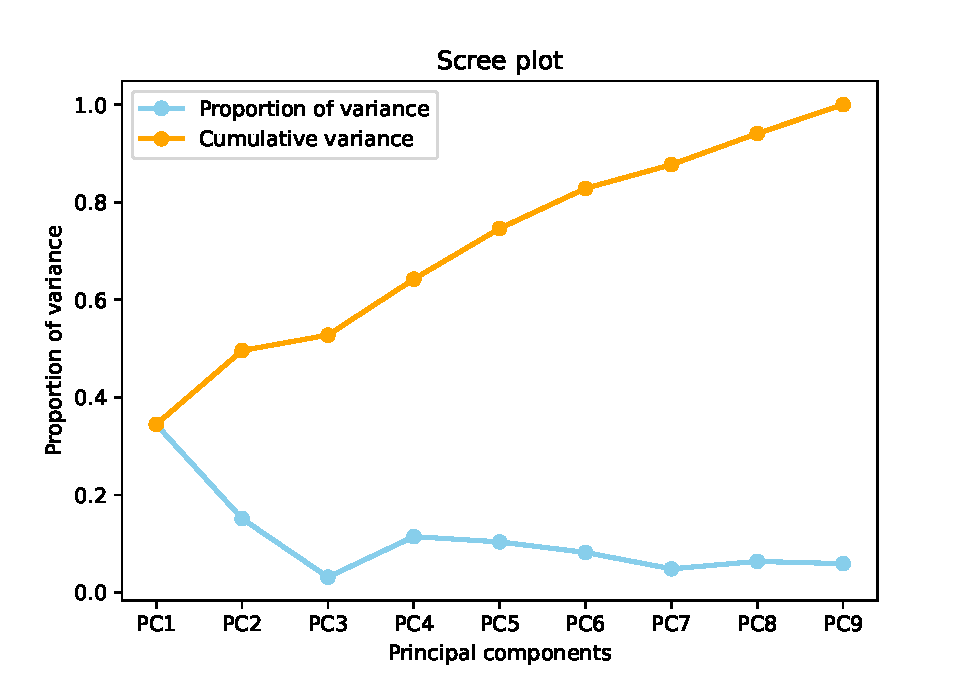
\includegraphics[keepaspectratio]{RandPytonAnalysisPDF_files/RandPytonAnalysisPDF_files/figure-latex/unnamed-chunk-8-1.pdf}}

\section{Collaboration R and python}\label{collaboration-r-and-python}

\url{https://rstudio.github.io/reticulate/}

\begin{Shaded}
\begin{Highlighting}[]
\NormalTok{library(reticulate)}
\NormalTok{library(ade4)}
\NormalTok{P \textless{}{-} py$P}
\NormalTok{colnames(P) \textless{}{-} paste("Axis",1:ncol(P),sep="")}
\NormalTok{rownames(P) \textless{}{-} colnames(py$deugtab)}
\NormalTok{par(mfrow=c(2,2))}
\NormalTok{s.corcircle(P,sub="Python version")}
\NormalTok{s.corcircle(pca2$c1,sub="R version")}
\NormalTok{plot(P[,1],pca2$c1[,1],panel.first=c(grid()),xlab="Python (axis 1)",}
\NormalTok{     ylab="R (axis 1)",pch=19);abline(0,{-}1,col="red")}
\NormalTok{plot(P[,2],pca2$c1[,2],panel.first=c(grid()),xlab="Python (axis 2)",}
\NormalTok{     ylab="R (axis 2)",pch=19);abline(0,{-}1,col="red")}
\end{Highlighting}
\end{Shaded}

\pandocbounded{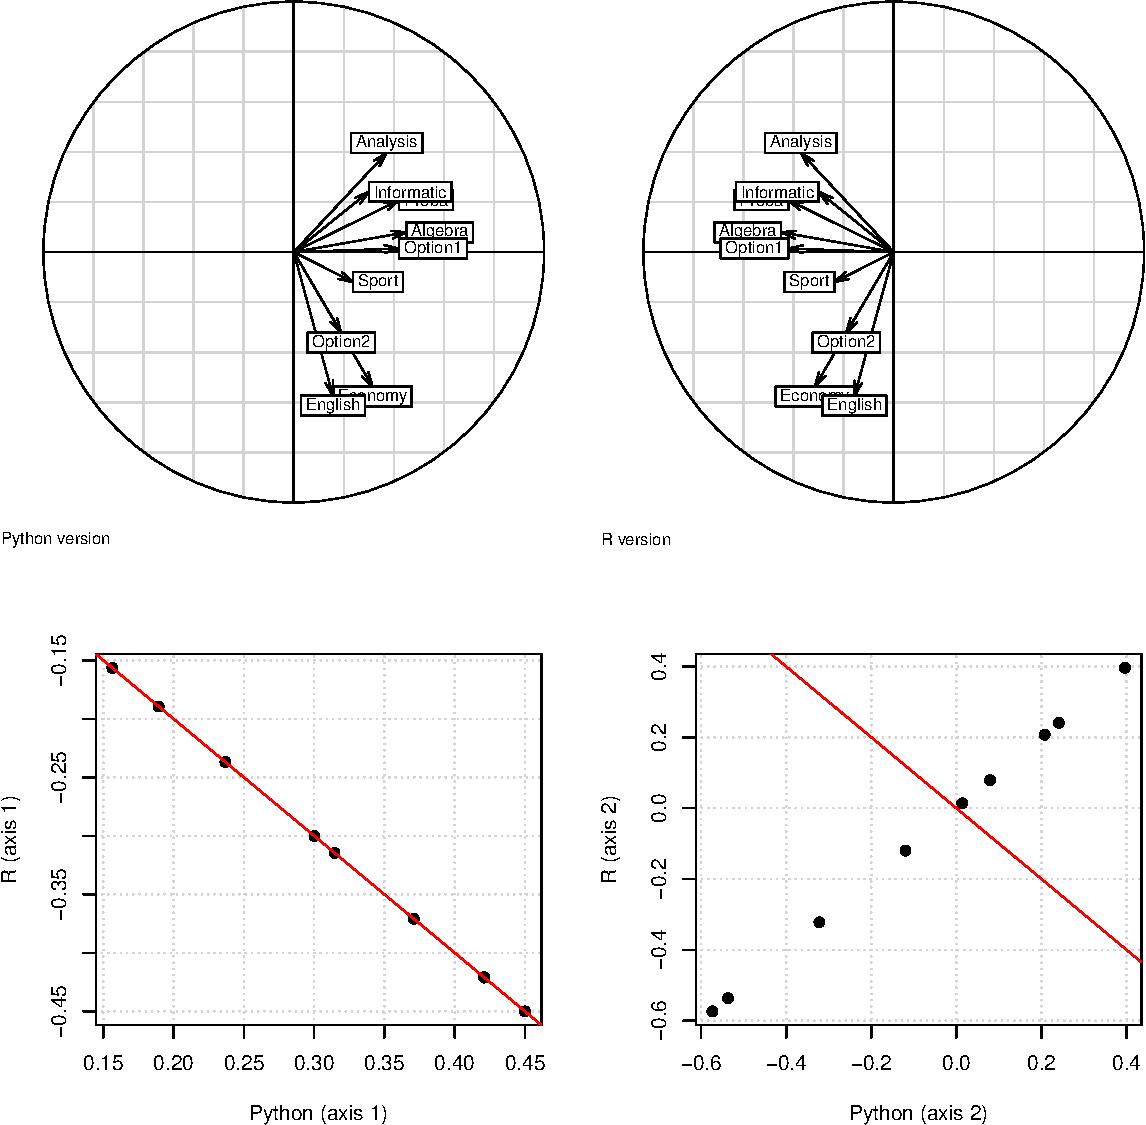
\includegraphics[keepaspectratio]{RandPytonAnalysisPDF_files/RandPytonAnalysisPDF_files/figure-latex/unnamed-chunk-9-3.pdf}}

\begin{Shaded}
\begin{Highlighting}[]
\NormalTok{coordli \textless{}{-} py$Z\_new}
\NormalTok{colnames(coordli) \textless{}{-} paste("CS",1:ncol(coordli),sep="")}
\NormalTok{rownames(coordli) \textless{}{-} rownames(py$deugtab)}
\NormalTok{par(mfrow=c(2,2))}
\NormalTok{s.label(coordli,sub="Python version")}
\NormalTok{s.label(pca2$li,sub="R version")}
\NormalTok{plot(coordli[,1],pca2$li[,1],panel.first=c(grid()),xlab="Python (CS 1)",}
\NormalTok{     ylab="R (CS 1)",pch=19);abline(0,{-}1,col="red")}
\NormalTok{plot(coordli[,2],pca2$li[,2],panel.first=c(grid()),xlab="Python (CS 2)",}
\NormalTok{     ylab="R (CS 2)",pch=19);abline(0,{-}1,col="red")}
\end{Highlighting}
\end{Shaded}

\pandocbounded{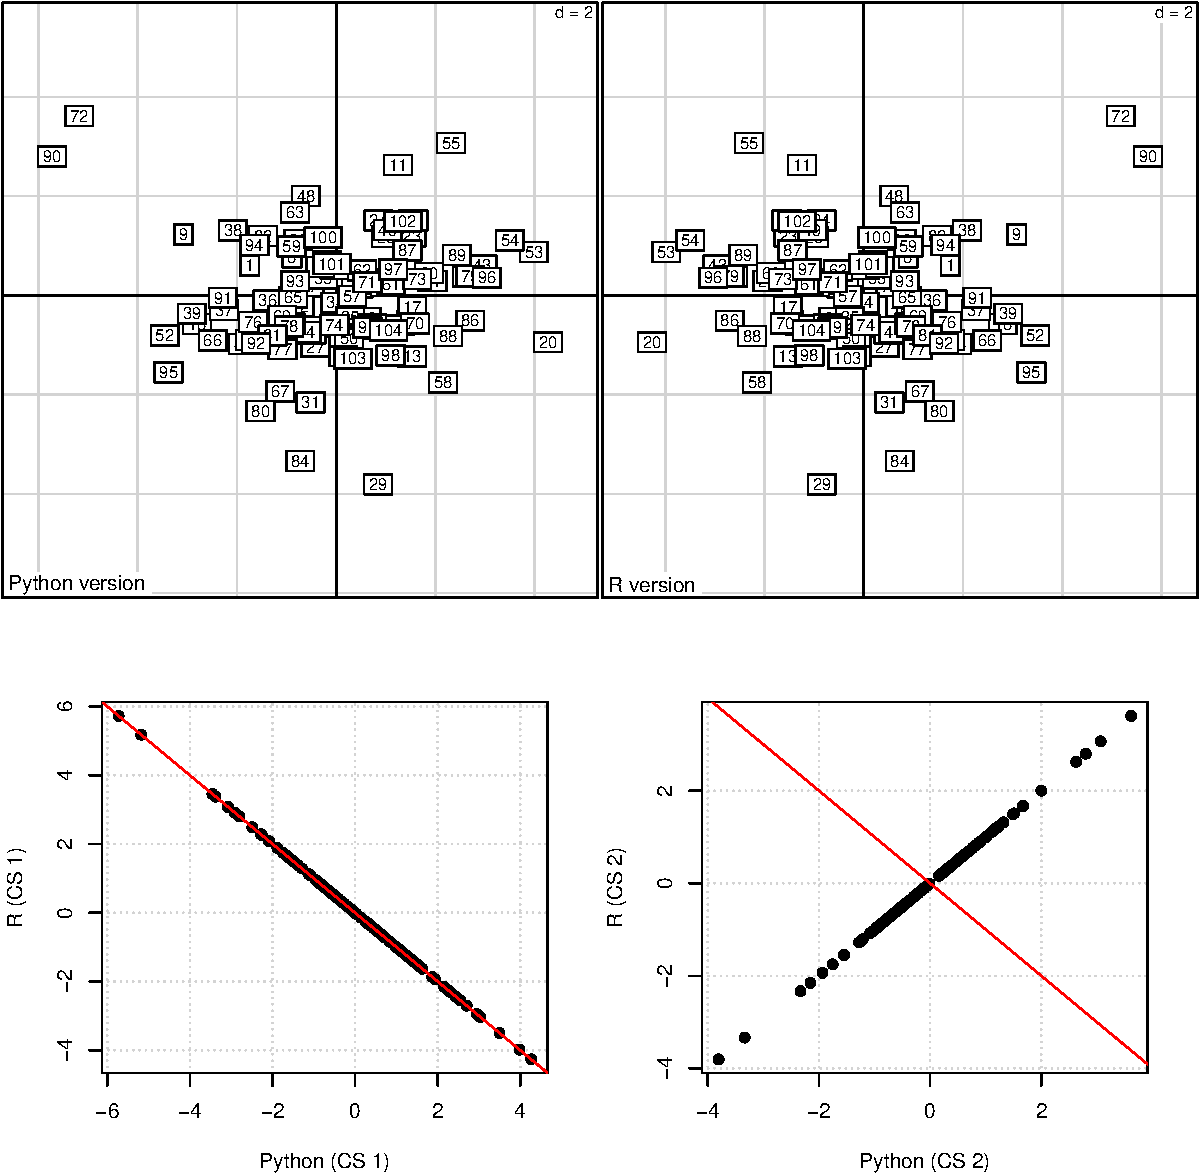
\includegraphics[keepaspectratio]{RandPytonAnalysisPDF_files/RandPytonAnalysisPDF_files/figure-latex/unnamed-chunk-10-1.pdf}}

\begin{Shaded}
\begin{Highlighting}[]
\NormalTok{par(mfrow=c(1,2))}
\NormalTok{plot(py$eigenvalues,pca2$eig,type="b",panel.first=c(grid()),pch=19)}
\NormalTok{abline(0,1,col="red")}
\NormalTok{plot(sort(py$eigenvalues,decreasing = TRUE),pca2$eig,type="b",}
\NormalTok{     panel.first=c(grid()),pch=19)}
\NormalTok{abline(0,1,col="red")}
\end{Highlighting}
\end{Shaded}

\pandocbounded{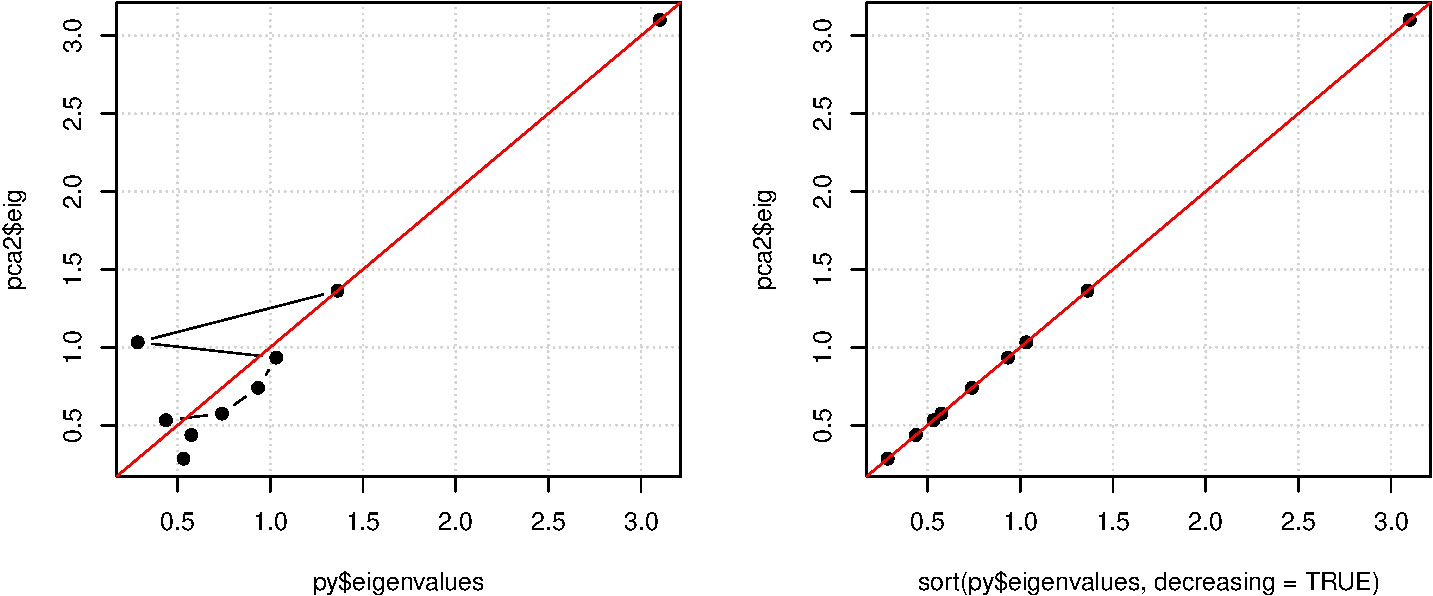
\includegraphics[keepaspectratio]{RandPytonAnalysisPDF_files/RandPytonAnalysisPDF_files/figure-latex/unnamed-chunk-11-1.pdf}}

problem in the order of the eigenvalues !!!

\begin{Shaded}
\begin{Highlighting}[]
\NormalTok{pca2$eig}
\end{Highlighting}
\end{Shaded}

\begin{verbatim}
## [1] 3.1013578 1.3629834 1.0323269 0.9340533 0.7397529 0.5746693 0.5325414 0.4375395
## [9] 0.2847754
\end{verbatim}

\begin{Shaded}
\begin{Highlighting}[]
\NormalTok{py$D}
\end{Highlighting}
\end{Shaded}

\begin{verbatim}
##           [,1]     [,2]      [,3]     [,4]      [,5]      [,6]      [,7]      [,8]
##  [1,] 3.101358 0.000000 0.0000000 0.000000 0.0000000 0.0000000 0.0000000 0.0000000
##  [2,] 0.000000 1.362983 0.0000000 0.000000 0.0000000 0.0000000 0.0000000 0.0000000
##  [3,] 0.000000 0.000000 0.2847754 0.000000 0.0000000 0.0000000 0.0000000 0.0000000
##  [4,] 0.000000 0.000000 0.0000000 1.032327 0.0000000 0.0000000 0.0000000 0.0000000
##  [5,] 0.000000 0.000000 0.0000000 0.000000 0.9340533 0.0000000 0.0000000 0.0000000
##  [6,] 0.000000 0.000000 0.0000000 0.000000 0.0000000 0.7397529 0.0000000 0.0000000
##  [7,] 0.000000 0.000000 0.0000000 0.000000 0.0000000 0.0000000 0.4375395 0.0000000
##  [8,] 0.000000 0.000000 0.0000000 0.000000 0.0000000 0.0000000 0.0000000 0.5746693
##  [9,] 0.000000 0.000000 0.0000000 0.000000 0.0000000 0.0000000 0.0000000 0.0000000
##            [,9]
##  [1,] 0.0000000
##  [2,] 0.0000000
##  [3,] 0.0000000
##  [4,] 0.0000000
##  [5,] 0.0000000
##  [6,] 0.0000000
##  [7,] 0.0000000
##  [8,] 0.0000000
##  [9,] 0.5325414
\end{verbatim}

\begin{Shaded}
\begin{Highlighting}[]
\NormalTok{py$eigenvalues}
\end{Highlighting}
\end{Shaded}

\begin{verbatim}
## [1] 3.1013578 1.3629834 0.2847754 1.0323269 0.9340533 0.7397529 0.4375395 0.5746693
## [9] 0.5325414
\end{verbatim}

problem !!!

test of the pca from scikit-learn

\begin{Shaded}
\begin{Highlighting}[]
\NormalTok{import sklearn.decomposition as sd}
\NormalTok{from sklearn.decomposition import PCA}
\NormalTok{pca = PCA(n\_components=9)}
\NormalTok{Z2 = Z/np.sqrt(104)}
\NormalTok{pca.fit(Z2)}
\end{Highlighting}
\end{Shaded}

\begin{verbatim}
## PCA(n_components=9)
\end{verbatim}

\begin{Shaded}
\begin{Highlighting}[]
\NormalTok{print(pca.explained\_variance\_ratio\_)}
\end{Highlighting}
\end{Shaded}

\begin{verbatim}
## [0.34459531 0.1514426  0.11470299 0.1037837  0.08219477 0.06385214
##  0.05917127 0.0486155  0.03164171]
\end{verbatim}

\begin{Shaded}
\begin{Highlighting}[]
\NormalTok{print(pca.singular\_values\_)}
\end{Highlighting}
\end{Shaded}

\begin{verbatim}
## [1.76106724 1.16746882 1.01603489 0.96646433 0.86008891 0.75806943
##  0.72975436 0.66146771 0.5336435 ]
\end{verbatim}

\begin{Shaded}
\begin{Highlighting}[]
\NormalTok{print(pca.singular\_values\_*pca.singular\_values\_)}
\end{Highlighting}
\end{Shaded}

\begin{verbatim}
## [3.10135782 1.36298344 1.0323269  0.9340533  0.73975293 0.57466926
##  0.53254143 0.43753953 0.28477539]
\end{verbatim}

\section{Construction of the function ``pydudi'' (first
prototype)}\label{construction-of-the-function-pydudi-first-prototype}

based on the duality diagram (see more details below)

\begin{itemize}
\tightlist
\item
  \url{https://pbil.univ-lyon1.fr/R/pdf/tdr61.pdf}
\item
  \url{https://pbil.univ-lyon1.fr/R/pdf/stage3.pdf}
\item
  \url{https://pbil.univ-lyon1.fr/R/pdf/bs8.pdf}
\end{itemize}

first test =\textgreater{} need to adjust the weighting (test with COA)

\begin{Shaded}
\begin{Highlighting}[]
\NormalTok{import os}
\NormalTok{import string}
\NormalTok{import re}
\NormalTok{import pandas as pd}
\NormalTok{import numpy as np}

\NormalTok{def pydudi(X,cw,lw,nf):}
\NormalTok{  dim = X.shape}
\NormalTok{  n = dim[0]}
\NormalTok{  p = dim[1]}
\NormalTok{  nf0 = nf{-}1}
\NormalTok{  \# n=len(X)}
\NormalTok{  \# p=len(X.columns)}
\NormalTok{  D = np.diag(np.sqrt(lw))}
\NormalTok{  Q = np.diag(np.sqrt(cw))}
  
\NormalTok{  \# XtDXQ =\textgreater{} problem  with Q !!!}
  
\NormalTok{  XD = np.dot(X.T,D).T}
\NormalTok{  XD = np.dot(XD,Q)}
\NormalTok{  XtX = np.dot(XD.T,XD)}
  
  
\NormalTok{  \# decomposition}
\NormalTok{  eigenvalues, eigenvectors = np.linalg.eig(XtX)}
\NormalTok{  index = np.argsort(eigenvalues)[::{-}1]}
  
\NormalTok{  \# np.nonzero(eigenvalues)[0]}
\NormalTok{  eigenvalues = eigenvalues.real}
\NormalTok{  eigenvectors = eigenvectors.real}
\NormalTok{  eigenvalues=eigenvalues[index]}
\NormalTok{  eigenvectors=eigenvectors[:,index]}
\NormalTok{  \# results}
\NormalTok{  rank = len(np.nonzero(eigenvalues)[0])}
\NormalTok{  C1 = np.dot(np.diag(1/np.sqrt(cw)),eigenvectors[:,0:nf])}
\NormalTok{  \#C1 = eigenvectors[:,0:nf]}
\NormalTok{  XQ = np.dot(X,np.diag(cw))}
\NormalTok{  Li = np.dot(XQ, C1)}
  
\NormalTok{  \# need to adjust the weighting (problem with sqrt)}
\NormalTok{  L1 = np.dot(Li,np.diag(1/np.sqrt(eigenvalues[0:nf])))}
\NormalTok{  Co = np.dot(C1,np.diag(np.sqrt(eigenvalues[0:nf])))}
\NormalTok{  return eigenvalues,rank,Li,L1,Co,C1,nf;}

\NormalTok{\#\#\#}
\end{Highlighting}
\end{Shaded}

\subsection{Test pydudi with PCA}\label{test-pydudi-with-pca}

\begin{Shaded}
\begin{Highlighting}[]
\NormalTok{import numpy as np }
\NormalTok{import pandas as pd}
\NormalTok{deugtab = pd.read\_csv(\textquotesingle{}data/deugtab.csv\textquotesingle{})}
\NormalTok{deugtab}
\end{Highlighting}
\end{Shaded}

\begin{verbatim}
##      Unnamed: 0  Algebra  Analysis  Proba  ...  Option1  Option2  English  Sport
## 0             1       40      26.0     26  ...       17     24.0     19.0   11.5
## 1             2       37      34.5     37  ...       24     22.0     26.0   11.5
## 2             3       37      41.0     29  ...       24     27.0     19.6   11.5
## 3             4       63      37.5     57  ...       23     23.0     21.0   14.0
## 4             5       55      31.5     34  ...       19     24.0     24.0   11.5
## ..          ...      ...       ...    ...  ...      ...      ...      ...    ...
## 99          100       60      41.0     18  ...       20     24.0     17.2    0.0
## 100         101       48      44.0     22  ...       22     28.0     19.6    0.0
## 101         102       44      45.0     42  ...       27     22.0     18.4   15.0
## 102         103       47      32.0     26  ...       23     28.0     19.0   11.5
## 103         104       44      32.0     42  ...       28     27.5     23.0   11.5
## 
## [104 rows x 10 columns]
\end{verbatim}

\begin{Shaded}
\begin{Highlighting}[]
\NormalTok{del deugtab[\textquotesingle{}Unnamed: 0\textquotesingle{}]}
\NormalTok{deugtab}
\end{Highlighting}
\end{Shaded}

\begin{verbatim}
##      Algebra  Analysis  Proba  Informatic  ...  Option1  Option2  English  Sport
## 0         40      26.0     26        26.0  ...       17     24.0     19.0   11.5
## 1         37      34.5     37        32.0  ...       24     22.0     26.0   11.5
## 2         37      41.0     29        34.5  ...       24     27.0     19.6   11.5
## 3         63      37.5     57        35.5  ...       23     23.0     21.0   14.0
## 4         55      31.5     34        36.0  ...       19     24.0     24.0   11.5
## ..       ...       ...    ...         ...  ...      ...      ...      ...    ...
## 99        60      41.0     18        30.0  ...       20     24.0     17.2    0.0
## 100       48      44.0     22        30.0  ...       22     28.0     19.6    0.0
## 101       44      45.0     42        35.0  ...       27     22.0     18.4   15.0
## 102       47      32.0     26        21.0  ...       23     28.0     19.0   11.5
## 103       44      32.0     42        26.5  ...       28     27.5     23.0   11.5
## 
## [104 rows x 9 columns]
\end{verbatim}

\begin{Shaded}
\begin{Highlighting}[]
\NormalTok{X= deugtab {-} deugtab.mean()}
\NormalTok{\# Normalize}
\NormalTok{X = X / X.std(ddof=0)}
\NormalTok{dim = X.shape}
\NormalTok{n = dim[0]}
\NormalTok{p = dim[1]}
\NormalTok{\# lw = pd.DataFrame(np.repeat(1/len(X),len(X)))[0]}
\NormalTok{\# cw = pd.DataFrame(np.repeat(1,len(X.columns)))[0]}
\NormalTok{lw = pd.DataFrame(np.repeat(1/n,n))[0]}
\NormalTok{cw = pd.DataFrame(np.repeat(1,p))[0]}
\NormalTok{ted = pydudi(X,cw,lw,2)}
\end{Highlighting}
\end{Shaded}

\begin{Shaded}
\begin{Highlighting}[]
\NormalTok{library(reticulate)}
\NormalTok{names(py$ted) \textless{}{-} c("eig","rank","li","l1","co","c1","nf")}
\NormalTok{coordli \textless{}{-} py$ted$li}
\NormalTok{par(mfrow=c(2,2))}
\NormalTok{s.label(coordli,sub="Python version")}
\NormalTok{s.label(pca2$li,sub="R version")}
\NormalTok{plot(coordli[,1],pca2$li[,1],panel.first=c(grid()),xlab="Python (CS 1)",}
\NormalTok{     ylab="R (CS 1)",pch=19);abline(0,{-}1,col="red")}
\NormalTok{plot(coordli[,2],pca2$li[,2],panel.first=c(grid()),xlab="Python (CS 2)",}
\NormalTok{     ylab="R (CS 2)",pch=19);abline(0,{-}1,col="red")}
\end{Highlighting}
\end{Shaded}

\pandocbounded{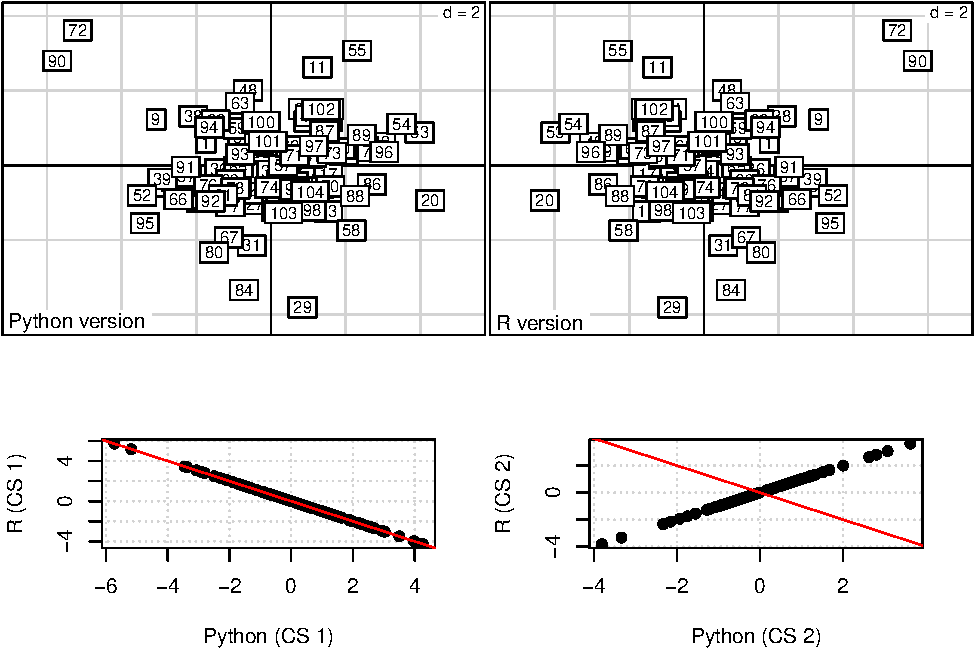
\includegraphics[keepaspectratio]{RandPytonAnalysisPDF_files/RandPytonAnalysisPDF_files/figure-latex/unnamed-chunk-16-1.pdf}}

\begin{Shaded}
\begin{Highlighting}[]
\NormalTok{coordl1 \textless{}{-} py$ted$l1}
\NormalTok{par(mfrow=c(2,2))}
\NormalTok{s.label(coordl1,sub="Python version")}
\NormalTok{s.label(pca2$l1,sub="R version")}
\NormalTok{plot(coordl1[,1],pca2$l1[,1],panel.first=c(grid()),xlab="Python (CS 1)",}
\NormalTok{     ylab="R (CS 1)",pch=19);abline(0,{-}1,col="red")}
\NormalTok{plot(coordl1[,2],pca2$l1[,2],panel.first=c(grid()),xlab="Python (CS 2)",}
\NormalTok{     ylab="R (CS 2)",pch=19);abline(0,{-}1,col="red")}
\end{Highlighting}
\end{Shaded}

\pandocbounded{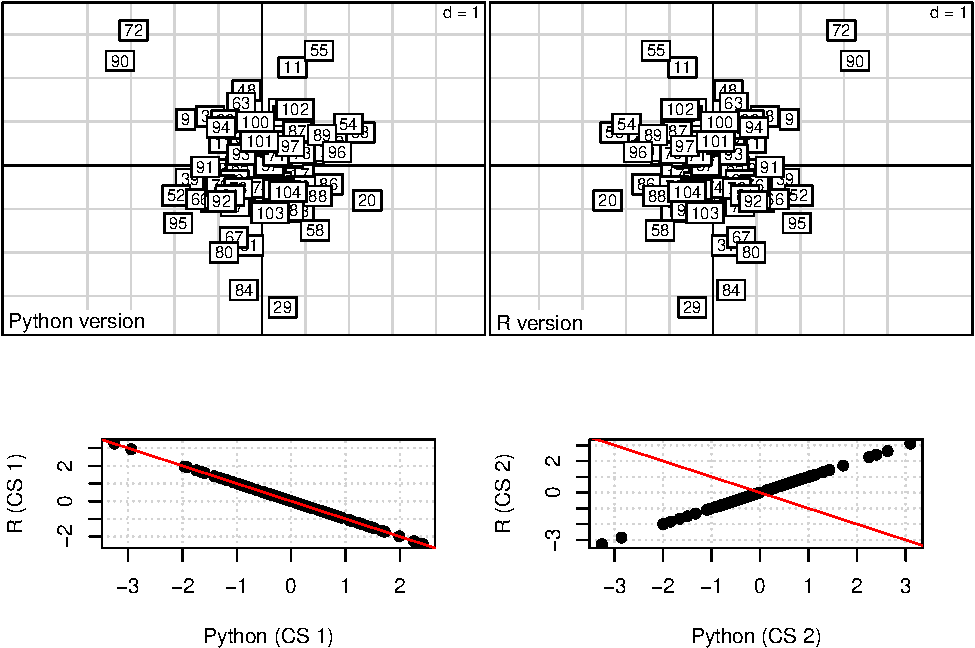
\includegraphics[keepaspectratio]{RandPytonAnalysisPDF_files/RandPytonAnalysisPDF_files/figure-latex/unnamed-chunk-17-1.pdf}}

\begin{Shaded}
\begin{Highlighting}[]
\NormalTok{par(mfrow=c(2,2))}
\NormalTok{s.corcircle(py$ted$co,sub="Python version")}
\NormalTok{s.corcircle(pca2$co,sub="R version")}
\NormalTok{plot(py$ted$c1[,1],pca2$c1[,1],panel.first=c(grid()),xlab="Python (axis 1)",}
\NormalTok{     ylab="R (axis 1)",pch=19);abline(0,{-}1,col="red")}
\NormalTok{plot(py$ted$c1[,2],pca2$c1[,2],panel.first=c(grid()),xlab="Python (axis 2)",}
\NormalTok{     ylab="R (axis 2)",pch=19);abline(0,{-}1,col="red")}
\end{Highlighting}
\end{Shaded}

\pandocbounded{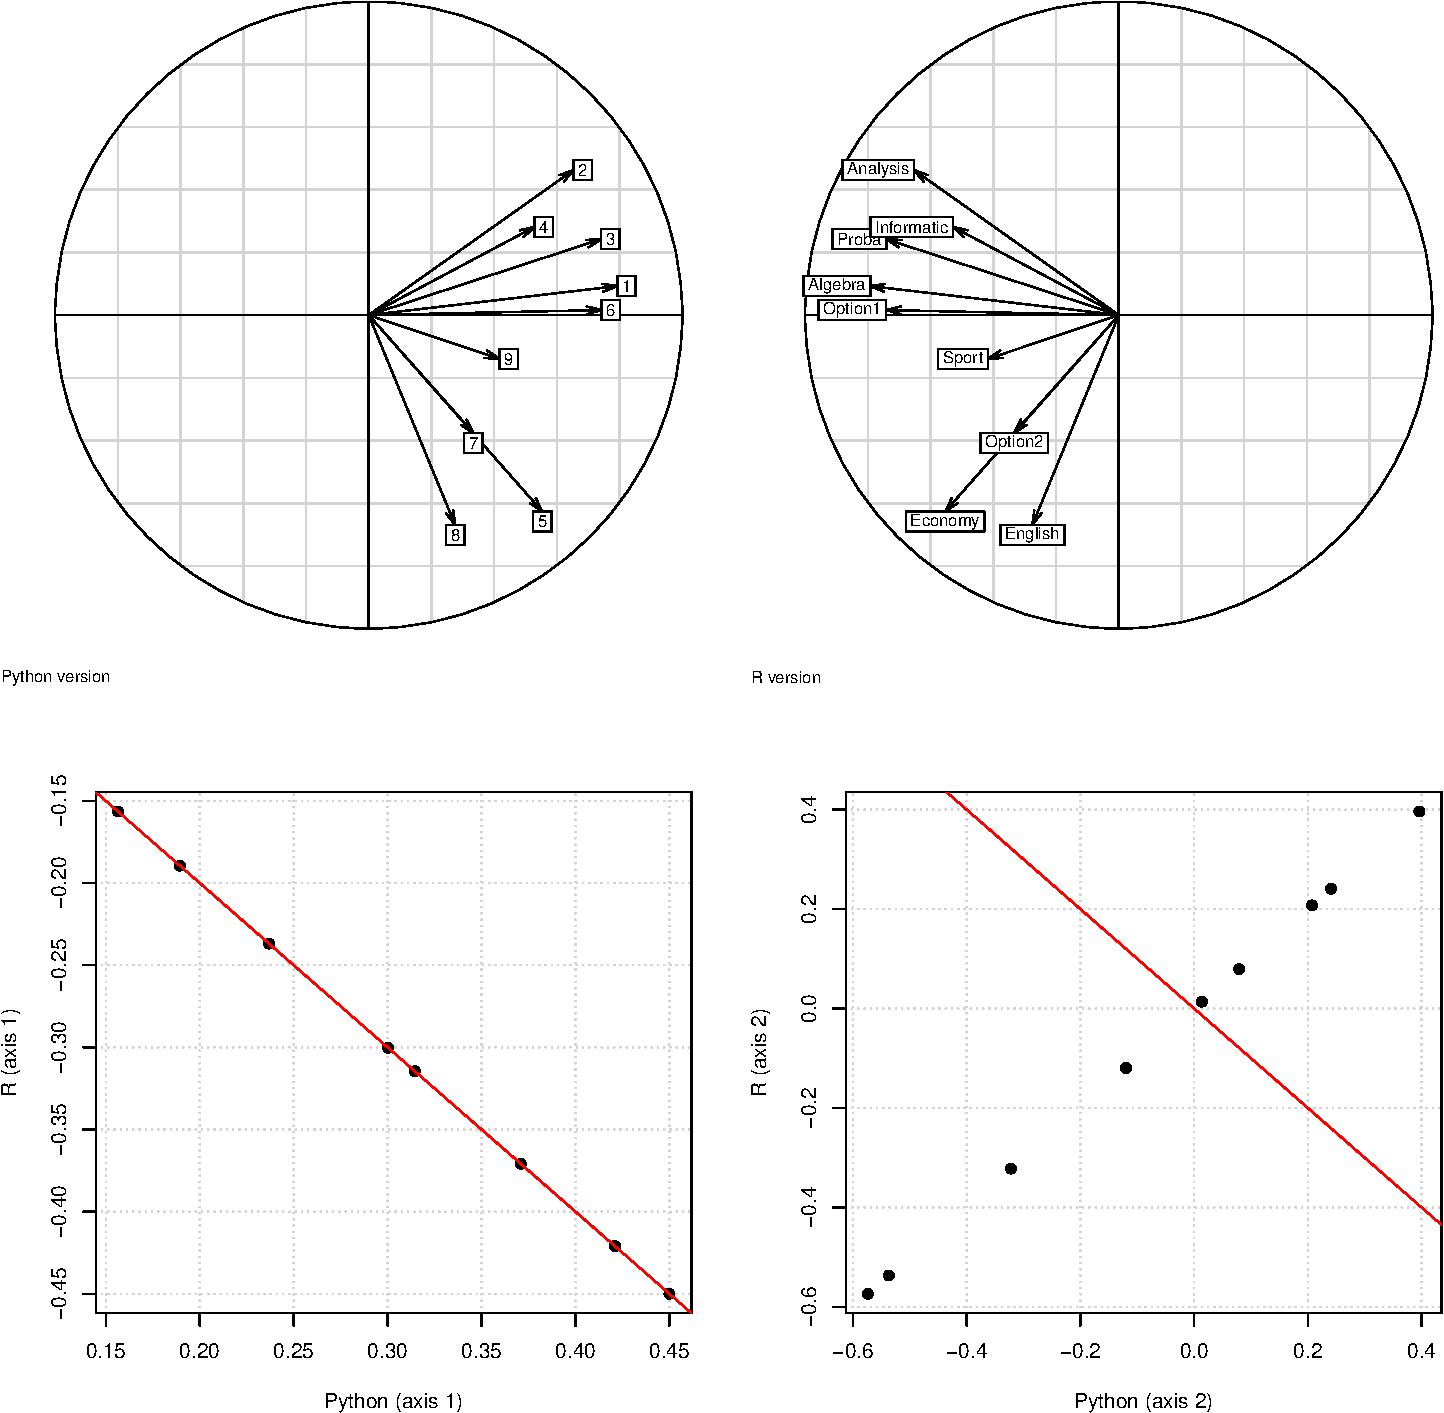
\includegraphics[keepaspectratio]{RandPytonAnalysisPDF_files/RandPytonAnalysisPDF_files/figure-latex/unnamed-chunk-18-1.pdf}}

\subsection{Test pydudi with COA}\label{test-pydudi-with-coa}

COA: correspondence analysis.

\begin{verbatim}
 Benzécri, J.P. and Coll. (1973) _L'analyse des données. II
 L'analyse des correspondances_, Bordas, Paris. 1-620.
 
 Greenacre, M. J. (1984) _Theory and applications of correspondence
 analysis_, Academic Press, London.
\end{verbatim}

Si R help from ade4 (dudi.coa) and
\url{https://pbil.univ-lyon1.fr/R/pdf/stage4.pdf}

\begin{Shaded}
\begin{Highlighting}[]
\NormalTok{data(rpjdl)}
\NormalTok{chisq.test(rpjdl$fau)$statistic}
\end{Highlighting}
\end{Shaded}

\begin{verbatim}
## Warning in chisq.test(rpjdl$fau): L’approximation du Chi-2 est peut-être incorrecte
\end{verbatim}

\begin{verbatim}
## X-squared 
##  7323.597
\end{verbatim}

\begin{Shaded}
\begin{Highlighting}[]
\NormalTok{rpjdl.coa \textless{}{-} coa1 \textless{}{-} dudi.coa(rpjdl$fau, scannf = FALSE, nf = 4)}
\NormalTok{sum(rpjdl.coa$eig)*rpjdl.coa$N \# the same}
\end{Highlighting}
\end{Shaded}

\begin{verbatim}
## [1] 7323.597
\end{verbatim}

\begin{Shaded}
\begin{Highlighting}[]
\NormalTok{write.csv(rpjdl$fau,file="data/fau.csv")}
\end{Highlighting}
\end{Shaded}

\begin{Shaded}
\begin{Highlighting}[]
\NormalTok{\# import numpy as np }
\NormalTok{import pandas as pd}
\NormalTok{fau = pd.read\_csv(\textquotesingle{}data/fau.csv\textquotesingle{})}
\NormalTok{fau}
\end{Highlighting}
\end{Shaded}

\begin{verbatim}
##      Unnamed: 0  AR  CP  ST  CC  UE  PV  JT  ...  CN  SS  FC  MC  EC  EH  El  PD
## 0             1   0   0   0   0   0   0   0  ...   1   0   0   0   0   0   0   1
## 1             2   0   0   0   0   0   0   0  ...   0   1   0   0   0   0   0   0
## 2             3   0   0   0   0   1   0   0  ...   1   1   0   0   0   0   1   0
## 3             4   0   0   0   0   0   0   0  ...   1   0   0   0   0   0   0   0
## 4             5   1   0   0   0   0   0   0  ...   0   0   0   0   0   0   0   0
## ..          ...  ..  ..  ..  ..  ..  ..  ..  ...  ..  ..  ..  ..  ..  ..  ..  ..
## 177         178   0   0   0   0   0   0   0  ...   0   0   0   0   0   0   0   0
## 178         179   0   0   0   0   0   0   0  ...   0   0   1   0   0   0   0   0
## 179         180   0   0   0   0   0   1   0  ...   0   1   1   0   0   0   0   0
## 180         181   0   0   1   0   0   0   1  ...   0   1   0   0   0   0   0   0
## 181         182   0   0   0   0   0   0   0  ...   0   1   1   0   1   0   0   0
## 
## [182 rows x 52 columns]
\end{verbatim}

\begin{Shaded}
\begin{Highlighting}[]
\NormalTok{del fau[\textquotesingle{}Unnamed: 0\textquotesingle{}]}
\NormalTok{fau}
\end{Highlighting}
\end{Shaded}

\begin{verbatim}
##      AR  CP  ST  CC  UE  PV  JT  GT  LA  ...  CA  CN  SS  FC  MC  EC  EH  El  PD
## 0     0   0   0   0   0   0   0   0   0  ...   1   1   0   0   0   0   0   0   1
## 1     0   0   0   0   0   0   0   1   0  ...   1   0   1   0   0   0   0   0   0
## 2     0   0   0   0   1   0   0   0   0  ...   0   1   1   0   0   0   0   1   0
## 3     0   0   0   0   0   0   0   0   0  ...   0   1   0   0   0   0   0   0   0
## 4     1   0   0   0   0   0   0   1   0  ...   1   0   0   0   0   0   0   0   0
## ..   ..  ..  ..  ..  ..  ..  ..  ..  ..  ...  ..  ..  ..  ..  ..  ..  ..  ..  ..
## 177   0   0   0   0   0   0   0   0   0  ...   0   0   0   0   0   0   0   0   0
## 178   0   0   0   0   0   0   0   0   0  ...   0   0   0   1   0   0   0   0   0
## 179   0   0   0   0   0   1   0   0   0  ...   0   0   1   1   0   0   0   0   0
## 180   0   0   1   0   0   0   1   0   0  ...   0   0   1   0   0   0   0   0   0
## 181   0   0   0   0   0   0   0   0   0  ...   0   0   1   1   0   1   0   0   0
## 
## [182 rows x 51 columns]
\end{verbatim}

\begin{Shaded}
\begin{Highlighting}[]
\NormalTok{import numpy as np}

\NormalTok{X=fau}
\NormalTok{sumX = fau.sum().sum()}
\NormalTok{sumCol =  fau.sum(axis=0)}
\NormalTok{sumRow = fau.sum(axis=1)}

\NormalTok{pij = X/sumX}
\NormalTok{pi = sumRow/sumX}
\NormalTok{pj = sumCol/sumX}

\NormalTok{Dj = np.diag(1/pj)}
\NormalTok{Di = np.diag(1/pi)}

\NormalTok{Z = np.dot(Di,pij)}
\NormalTok{Z= np.dot(Z,Dj)}
\NormalTok{Z.shape}
\end{Highlighting}
\end{Shaded}

\begin{verbatim}
## (182, 51)
\end{verbatim}

\begin{Shaded}
\begin{Highlighting}[]
\NormalTok{Z =Z {-} 1}
\NormalTok{Z = np.nan\_to\_num(Z)}

\NormalTok{\# Normalize}
\NormalTok{lw = pi}
\NormalTok{cw = pj}
\NormalTok{D= np.diag(np.sqrt(pi))}
\NormalTok{Q= np.diag(np.sqrt(pj))}
\NormalTok{X =Z}
\NormalTok{ted = pydudi(Z,cw,lw,2)}
\end{Highlighting}
\end{Shaded}

\begin{Shaded}
\begin{Highlighting}[]
\NormalTok{require(reticulate)}
\NormalTok{names(py$ted) \textless{}{-} c("eig","rank","li","l1","co","c1","nf")}
\end{Highlighting}
\end{Shaded}

\begin{Shaded}
\begin{Highlighting}[]
\NormalTok{head(t(t(py$X)\%*\%py$D))[,1]}
\end{Highlighting}
\end{Shaded}

\begin{verbatim}
## [1] -0.06986433 -0.06986433 -0.06535210 -0.04940154  0.85002979  0.76588343
\end{verbatim}

\begin{Shaded}
\begin{Highlighting}[]
\NormalTok{head(py$X*diag(py$D))[,1]}
\end{Highlighting}
\end{Shaded}

\begin{verbatim}
## [1] -0.06986433 -0.06986433 -0.06535210 -0.04940154  0.85002979  0.76588343
\end{verbatim}

\begin{Shaded}
\begin{Highlighting}[]
\NormalTok{XD \textless{}{-} t(t(py$X)\%*\%py$D)}
\NormalTok{head(XD\%*\%py$Q)[,1]}
\end{Highlighting}
\end{Shaded}

\begin{verbatim}
## [1] -0.007717578 -0.007717578 -0.007219133 -0.005457152  0.093898719  0.084603474
\end{verbatim}

\begin{Shaded}
\begin{Highlighting}[]
\NormalTok{head(sweep(XD,2,diag(py$Q),"*"))[,1]}
\end{Highlighting}
\end{Shaded}

\begin{verbatim}
## [1] -0.007717578 -0.007717578 -0.007219133 -0.005457152  0.093898719  0.084603474
\end{verbatim}

\begin{Shaded}
\begin{Highlighting}[]
\NormalTok{coa1$eig}
\end{Highlighting}
\end{Shaded}

\begin{verbatim}
##  [1] 0.753246079 0.292905714 0.229339077 0.204667043 0.157288711 0.151440858
##  [7] 0.150767524 0.139271459 0.128099632 0.121613888 0.117678929 0.114349277
## [13] 0.111133629 0.108686867 0.104567293 0.098786861 0.093491391 0.089476206
## [19] 0.083038229 0.078627728 0.071855317 0.066171912 0.064569801 0.063747501
## [25] 0.061830129 0.056205831 0.054891709 0.051264371 0.051057282 0.048112526
## [31] 0.047741238 0.045225569 0.042174679 0.041081123 0.039945517 0.037205530
## [37] 0.034420610 0.031713688 0.029256753 0.027162167 0.026386209 0.022092347
## [43] 0.021089820 0.020517411 0.016786030 0.016066325 0.015476722 0.014463573
## [49] 0.012991222 0.008353461
\end{verbatim}

\begin{Shaded}
\begin{Highlighting}[]
\NormalTok{py$ted$eig}
\end{Highlighting}
\end{Shaded}

\begin{verbatim}
##  [1]  7.532461e-01  2.929057e-01  2.293391e-01  2.046670e-01  1.572887e-01
##  [6]  1.514409e-01  1.507675e-01  1.392715e-01  1.280996e-01  1.216139e-01
## [11]  1.176789e-01  1.143493e-01  1.111336e-01  1.086869e-01  1.045673e-01
## [16]  9.878686e-02  9.349139e-02  8.947621e-02  8.303823e-02  7.862773e-02
## [21]  7.185532e-02  6.617191e-02  6.456980e-02  6.374750e-02  6.183013e-02
## [26]  5.620583e-02  5.489171e-02  5.126437e-02  5.105728e-02  4.811253e-02
## [31]  4.774124e-02  4.522557e-02  4.217468e-02  4.108112e-02  3.994552e-02
## [36]  3.720553e-02  3.442061e-02  3.171369e-02  2.925675e-02  2.716217e-02
## [41]  2.638621e-02  2.209235e-02  2.108982e-02  2.051741e-02  1.678603e-02
## [46]  1.606633e-02  1.547672e-02  1.446357e-02  1.299122e-02  8.353461e-03
## [51] -1.964766e-17
\end{verbatim}

ok for the eigenvalues, probleme dans le calcul des coordonnées ???

\begin{Shaded}
\begin{Highlighting}[]
\NormalTok{coordli \textless{}{-} py$ted$li}
\NormalTok{par(mfrow=c(2,2))}
\NormalTok{s.label(coordli,sub="Python version")}
\NormalTok{s.label(coa1$li,sub="R version")}
\NormalTok{plot(coordli[,1],coa1$li[,1],panel.first=c(grid()),xlab="Python (CS 1)",}
\NormalTok{     ylab="R (CS 1)",pch=19);abline(0,{-}1,col="red")}
\NormalTok{plot(coordli[,2],coa1$li[,2],panel.first=c(grid()),xlab="Python (CS 2)",}
\NormalTok{     ylab="R (CS 2)",pch=19);abline(0,{-}1,col="red")}
\end{Highlighting}
\end{Shaded}

\pandocbounded{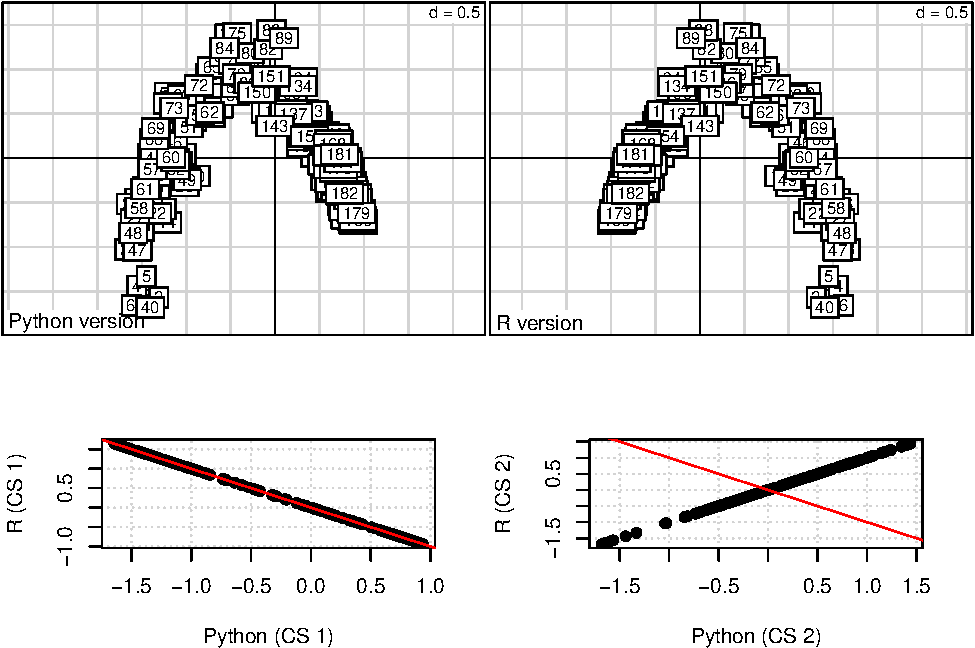
\includegraphics[keepaspectratio]{RandPytonAnalysisPDF_files/RandPytonAnalysisPDF_files/figure-latex/unnamed-chunk-27-1.pdf}}

\begin{Shaded}
\begin{Highlighting}[]
\NormalTok{coordl1 \textless{}{-} py$ted$l1}
\NormalTok{par(mfrow=c(2,2))}
\NormalTok{s.label(coordl1,sub="Python version")}
\NormalTok{s.label(coa1$l1,sub="R version")}
\NormalTok{plot(coordl1[,1],coa1$l1[,1],panel.first=c(grid()),xlab="Python (CS 1)",}
\NormalTok{     ylab="R (CS 1)",pch=19);abline(0,{-}1,col="red")}
\NormalTok{plot(coordl1[,2],coa1$l1[,2],panel.first=c(grid()),xlab="Python (CS 2)",}
\NormalTok{     ylab="R (CS 2)",pch=19);abline(0,{-}1,col="red")}
\end{Highlighting}
\end{Shaded}

\pandocbounded{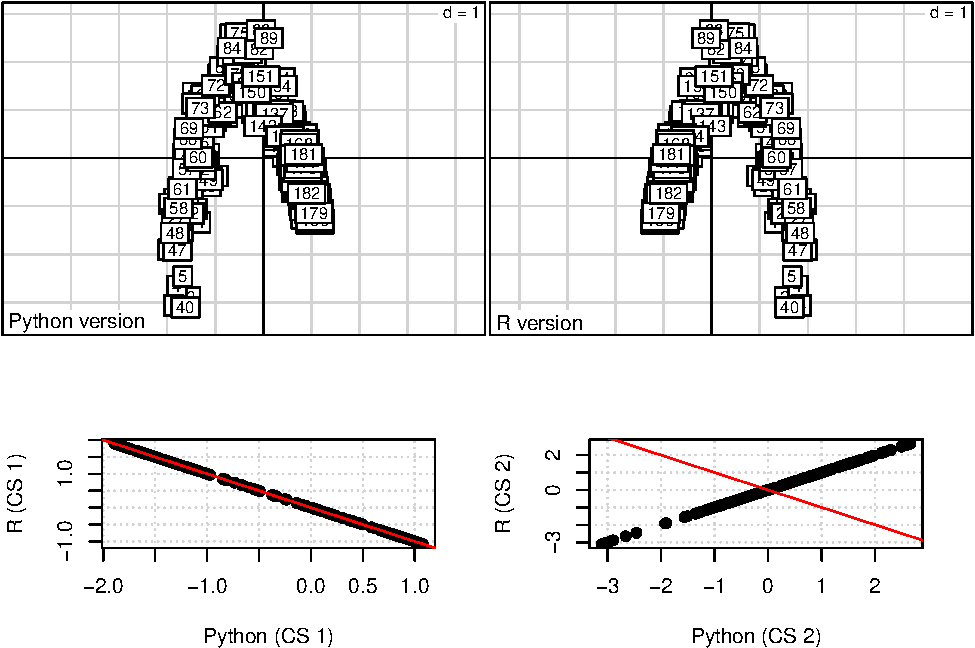
\includegraphics[keepaspectratio]{RandPytonAnalysisPDF_files/RandPytonAnalysisPDF_files/figure-latex/unnamed-chunk-28-1.pdf}}

\begin{Shaded}
\begin{Highlighting}[]
\NormalTok{par(mfrow=c(2,2))}
\NormalTok{plot(py$Z[,1],coa1$tab[,1],panel.first=c(grid()),xlab="Python (col 1 of Z)",}
\NormalTok{     ylab="R (col 1 of tab)",pch=19);abline(0,1,col="red")}
\NormalTok{plot(py$ted$c1[,1],coa1$c1[,1],panel.first=c(grid()),xlab="Python (normed Axis 1)",}
\NormalTok{     ylab="R (normed Axis 1)",pch=19);abline(0,{-}1,col="red")}
\NormalTok{plot(py$ted$co[,1],coa1$co[,1],panel.first=c(grid()),xlab="Python (Axis 1)",}
\NormalTok{     ylab="R (Axis 1)",pch=19);abline(0,{-}1,col="red")}
\end{Highlighting}
\end{Shaded}

\pandocbounded{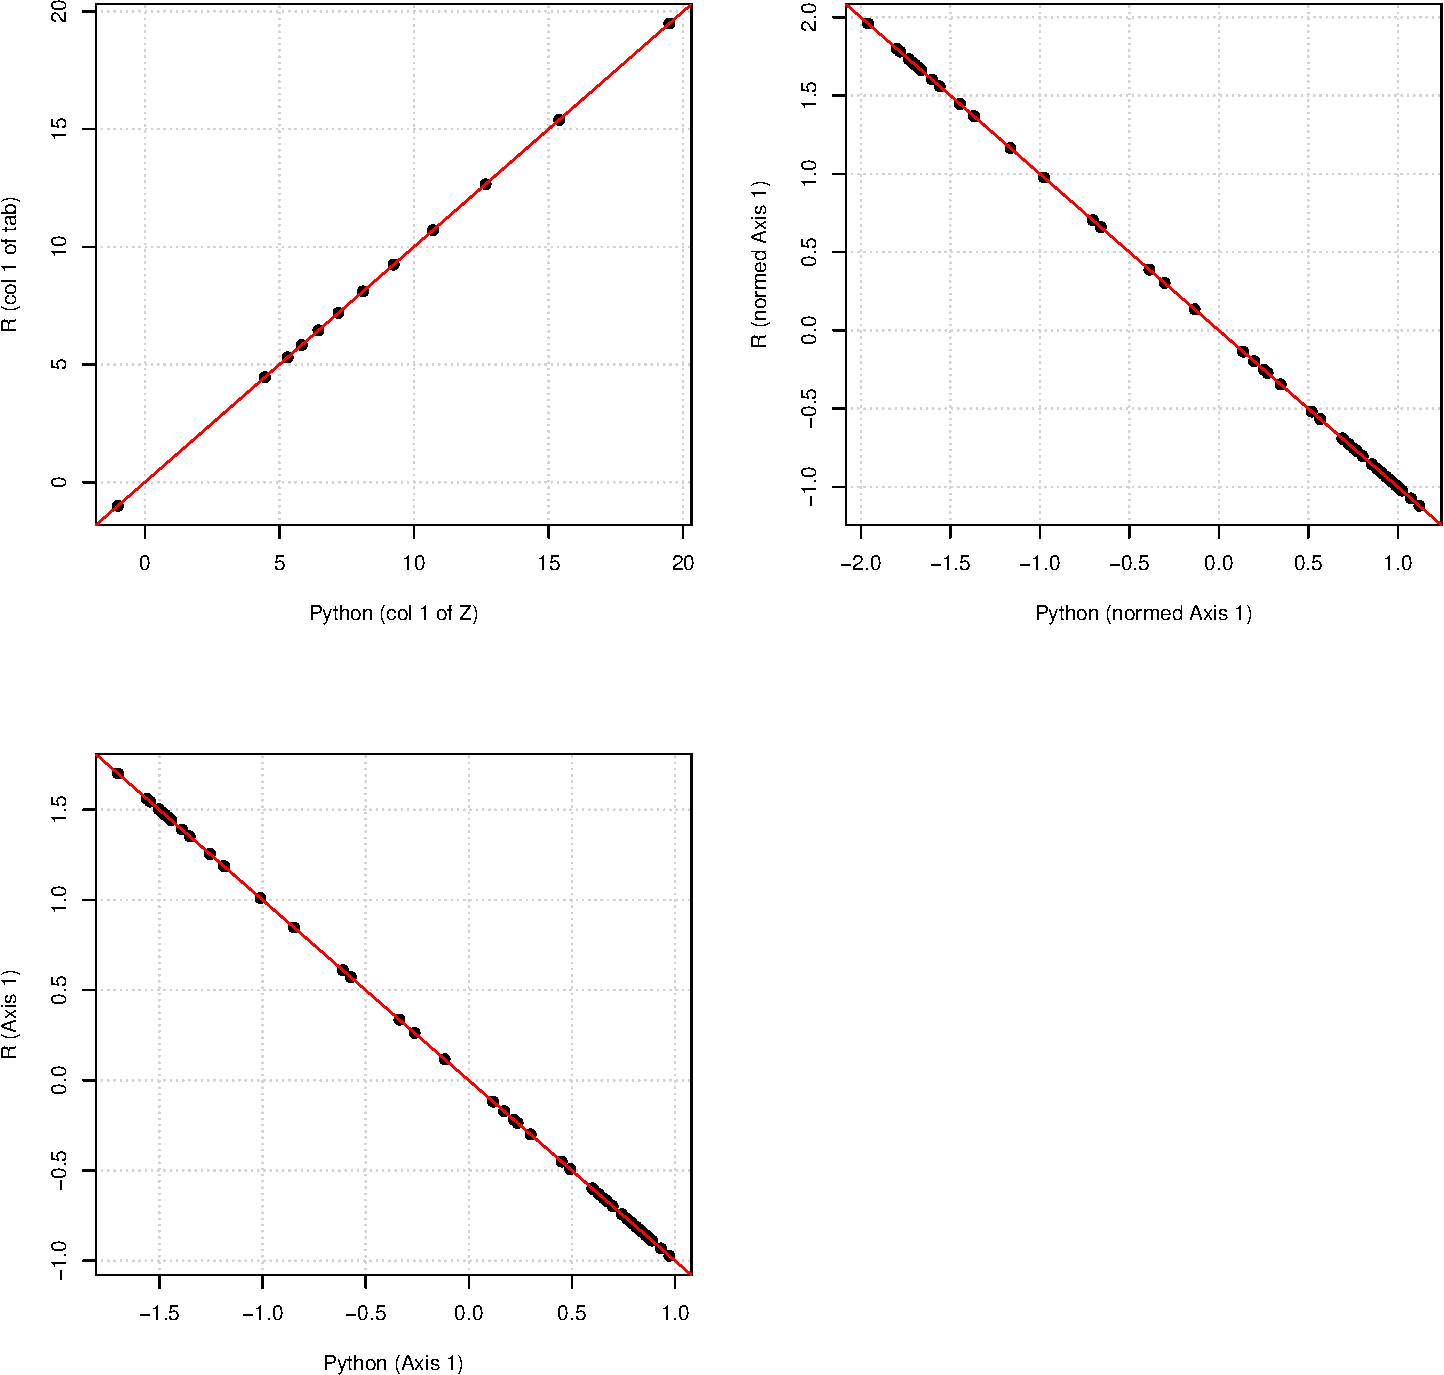
\includegraphics[keepaspectratio]{RandPytonAnalysisPDF_files/RandPytonAnalysisPDF_files/figure-latex/unnamed-chunk-29-1.pdf}}

=\textgreater{} need to check the weight !!! =\textgreater{} Ok !!

\subsection{Test pydudi with MCA}\label{test-pydudi-with-mca}

MCA: Multiple Correspondence Analysis

\begin{verbatim}
Tenenhaus, M. & Young, F.W. (1985) An analysis and synthesis of multiple correspondence analysis, optimal scaling, dual scaling, homogeneity analysis ans other     methods for quantifying categorical multivariate data. Psychometrika, 50, 1, 91-119.
Lebart, L., A. Morineau, and M. Piron. 1995. Statistique exploratoire multidimensionnelle. Dunod, Paris.
\end{verbatim}

Si R help from ade4 (dudi.acm) and
\url{https://pbil.univ-lyon1.fr/R/pdf/stage4.pdf}. the description of
the methods is given below:

\begin{itemize}
\tightlist
\item
  \url{https://pbil.univ-lyon1.fr/R/pdf/tdr521.pdf}
\item
  \url{https://pbil.univ-lyon1.fr/R/pdf/tdr52.pdf}
\end{itemize}

duality diagram

\begin{Shaded}
\begin{Highlighting}[]
\NormalTok{data(ours)}
\NormalTok{summary(ours)}
\end{Highlighting}
\end{Shaded}

\begin{verbatim}
##  altit  deniv  cloiso domain boise  hetra  favor  inexp  citat  depart 
##  1: 8   1:13   1:12   1: 9   1:10   1:19   1:15   1:20   1:22   AHP:5  
##  2:17   2:14   2: 4   2:13   2:15   2: 5   2:12   2:10   2: 7   AM :4  
##  3:13   3:11   3:22   3:16   3:13   3:14   3:11   3: 8   3: 4   D  :5  
##                                                          4: 5   HP :8  
##                                                                 HS :4  
##                                                                 I  :5  
##                                                                 S  :7
\end{verbatim}

\begin{Shaded}
\begin{Highlighting}[]
\NormalTok{acm1 \textless{}{-} dudi.acm(ours, scan = FALSE)}
\end{Highlighting}
\end{Shaded}

\begin{Shaded}
\begin{Highlighting}[]
\NormalTok{write.csv(ours,file="data/ours.csv")}
\end{Highlighting}
\end{Shaded}

importation with pandas

\begin{Shaded}
\begin{Highlighting}[]
\NormalTok{\# import numpy as np }
\NormalTok{import pandas as pd}
\NormalTok{ours = pd.read\_csv(\textquotesingle{}data/ours.csv\textquotesingle{})}
\NormalTok{ours}
\end{Highlighting}
\end{Shaded}

\begin{verbatim}
##     Unnamed: 0  altit  deniv  cloiso  domain  ...  hetra  favor  inexp  citat  depart
## 0            1      2      3       3       2  ...      3      3      2      1      HS
## 1            2      1      2       1       2  ...      1      2      2      2      HS
## 2            3      3      3       3       2  ...      2      3      3      2      HS
## 3            4      3      3       3       1  ...      3      3      2      3      HS
## 4            5      3      3       1       2  ...      3      2      3      1       S
## 5            6      3      3       3       1  ...      3      3      3      3       S
## 6            7      2      2       3       2  ...      1      2      3      1       S
## 7            8      1      1       2       2  ...      1      3      2      2       S
## 8            9      2      3       1       2  ...      2      3      3      4       S
## 9           10      2      2       3       1  ...      3      2      3      1       S
## 10          11      1      1       1       1  ...      1      2      2      1       S
## 11          12      2      2       3       1  ...      3      3      2      3       I
## 12          13      2      3       3       1  ...      3      3      2      3       I
## 13          14      1      3       2       2  ...      1      1      3      2       I
## 14          15      2      2       1       3  ...      2      2      2      1       I
## 15          16      3      3       3       3  ...      3      3      3      4       I
## 16          17      3      1       3       3  ...      3      3      1      4       D
## 17          18      3      2       3       3  ...      3      2      2      4       D
## 18          19      2      1       1       3  ...      3      3      1      4       D
## 19          20      2      1       1       2  ...      2      1      1      2       D
## 20          21      2      1       1       2  ...      2      1      1      1       D
## 21          22      1      1       1       2  ...      1      1      1      2      HP
## 22          23      2      2       2       2  ...      1      1      1      2      HP
## 23          24      1      1       3       3  ...      1      1      1      1      HP
## 24          25      2      3       2       3  ...      1      1      1      1      HP
## 25          26      2      2       1       1  ...      1      1      1      1      HP
## 26          27      2      2       3       1  ...      1      1      1      1      HP
## 27          28      3      2       1       3  ...      3      2      1      1      HP
## 28          29      2      1       1       2  ...      1      1      1      1      HP
## 29          30      1      1       3       3  ...      1      2      1      1     AHP
## 30          31      3      1       3       3  ...      3      2      1      1     AHP
## 31          32      3      2       3       3  ...      1      2      1      1     AHP
## 32          33      3      2       3       3  ...      1      1      1      1     AHP
## 33          34      3      1       3       1  ...      3      1      1      1     AHP
## 34          35      1      2       3       3  ...      1      1      1      1      AM
## 35          36      2      2       3       3  ...      1      1      1      1      AM
## 36          37      3      1       3       3  ...      1      1      1      1      AM
## 37          38      2      3       3       3  ...      1      2      2      1      AM
## 
## [38 rows x 11 columns]
\end{verbatim}

\begin{Shaded}
\begin{Highlighting}[]
\NormalTok{del ours[\textquotesingle{}Unnamed: 0\textquotesingle{}]}
\NormalTok{ours}
\end{Highlighting}
\end{Shaded}

\begin{verbatim}
##     altit  deniv  cloiso  domain  boise  hetra  favor  inexp  citat depart
## 0       2      3       3       2      2      3      3      2      1     HS
## 1       1      2       1       2      1      1      2      2      2     HS
## 2       3      3       3       2      2      2      3      3      2     HS
## 3       3      3       3       1      3      3      3      2      3     HS
## 4       3      3       1       2      2      3      2      3      1      S
## 5       3      3       3       1      3      3      3      3      3      S
## 6       2      2       3       2      2      1      2      3      1      S
## 7       1      1       2       2      1      1      3      2      2      S
## 8       2      3       1       2      3      2      3      3      4      S
## 9       2      2       3       1      3      3      2      3      1      S
## 10      1      1       1       1      1      1      2      2      1      S
## 11      2      2       3       1      3      3      3      2      3      I
## 12      2      3       3       1      3      3      3      2      3      I
## 13      1      3       2       2      1      1      1      3      2      I
## 14      2      2       1       3      2      2      2      2      1      I
## 15      3      3       3       3      3      3      3      3      4      I
## 16      3      1       3       3      3      3      3      1      4      D
## 17      3      2       3       3      3      3      2      2      4      D
## 18      2      1       1       3      3      3      3      1      4      D
## 19      2      1       1       2      2      2      1      1      2      D
## 20      2      1       1       2      2      2      1      1      1      D
## 21      1      1       1       2      1      1      1      1      2     HP
## 22      2      2       2       2      1      1      1      1      2     HP
## 23      1      1       3       3      1      1      1      1      1     HP
## 24      2      3       2       3      2      1      1      1      1     HP
## 25      2      2       1       1      2      1      1      1      1     HP
## 26      2      2       3       1      1      1      1      1      1     HP
## 27      3      2       1       3      3      3      2      1      1     HP
## 28      2      1       1       2      2      1      1      1      1     HP
## 29      1      1       3       3      1      1      2      1      1    AHP
## 30      3      1       3       3      2      3      2      1      1    AHP
## 31      3      2       3       3      2      1      2      1      1    AHP
## 32      3      2       3       3      2      1      1      1      1    AHP
## 33      3      1       3       1      3      3      1      1      1    AHP
## 34      1      2       3       3      1      1      1      1      1     AM
## 35      2      2       3       3      2      1      1      1      1     AM
## 36      3      1       3       3      3      1      1      1      1     AM
## 37      2      3       3       3      2      1      2      2      1     AM
\end{verbatim}

\begin{Shaded}
\begin{Highlighting}[]
\NormalTok{def disjonctif(X):}
\NormalTok{  X\_cat = X.astype("category")}
\NormalTok{  X\_dis = pd.get\_dummies(X\_cat)}
\NormalTok{  X\_dis = X\_dis*1}
\NormalTok{  return X\_dis ;}
\end{Highlighting}
\end{Shaded}

preparation of the triplet

\begin{Shaded}
\begin{Highlighting}[]
\NormalTok{Xdis = disjonctif(ours)}
\NormalTok{m = Xdis.shape[1]}
\NormalTok{n = Xdis.shape[0]}
\NormalTok{v = ours.shape[1]}
\NormalTok{lw = pd.DataFrame(np.repeat(1/n,n))[0]}
\NormalTok{D = np.diag(lw)}
\NormalTok{cw = np.dot(np.dot(Xdis.T,D), np.ones(n)) }
\NormalTok{Dm = np.diag(cw)}
\NormalTok{X = np.dot(Xdis,np.diag(1/cw)){-}1}
\NormalTok{cw = cw/v}
\NormalTok{ted = pydudi(X,cw,lw,2)}
\end{Highlighting}
\end{Shaded}

\begin{Shaded}
\begin{Highlighting}[]
\NormalTok{require(reticulate)}
\NormalTok{names(py$ted) \textless{}{-} c("eig","rank","li","l1","co","c1","nf")}
\end{Highlighting}
\end{Shaded}

\begin{Shaded}
\begin{Highlighting}[]
\NormalTok{coordli \textless{}{-} py$ted$li}
\NormalTok{par(mfrow=c(2,2))}
\NormalTok{s.label(coordli,sub="Python version")}
\NormalTok{s.label(acm1$li,sub="R version")}
\NormalTok{plot(coordli[,1],acm1$li[,1],panel.first=c(grid()),xlab="Python (CS 1)",}
\NormalTok{     ylab="R (CS 1)",pch=19);abline(0,1,col="red")}
\NormalTok{plot(coordli[,2],acm1$li[,2],panel.first=c(grid()),xlab="Python (CS 2)",}
\NormalTok{     ylab="R (CS 2)",pch=19);abline(0,{-}1,col="red")}
\end{Highlighting}
\end{Shaded}

\pandocbounded{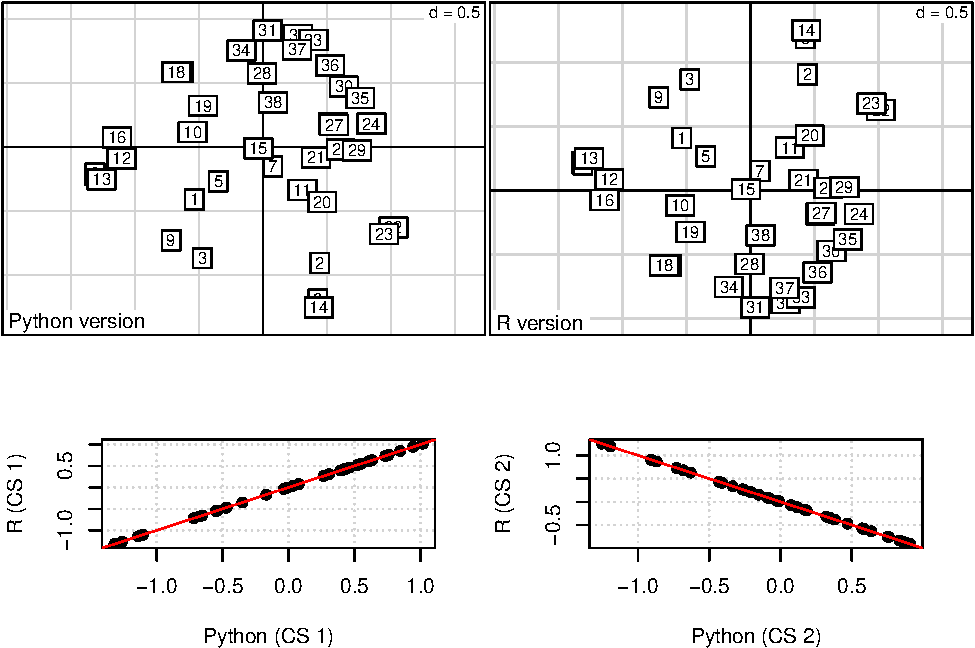
\includegraphics[keepaspectratio]{RandPytonAnalysisPDF_files/RandPytonAnalysisPDF_files/figure-latex/unnamed-chunk-36-1.pdf}}

\begin{Shaded}
\begin{Highlighting}[]
\NormalTok{coordl1 \textless{}{-} py$ted$l1}
\NormalTok{par(mfrow=c(2,2))}
\NormalTok{s.label(coordl1,sub="Python version")}
\NormalTok{s.label(acm1$l1,sub="R version")}
\NormalTok{plot(coordl1[,1],acm1$l1[,1],panel.first=c(grid()),xlab="Python (CS 1)",}
\NormalTok{     ylab="R (CS 1)",pch=19);abline(0,1,col="red")}
\NormalTok{plot(coordl1[,2],acm1$l1[,2],panel.first=c(grid()),xlab="Python (CS 2)",}
\NormalTok{     ylab="R (CS 2)",pch=19);abline(0,{-}1,col="red")}
\end{Highlighting}
\end{Shaded}

\pandocbounded{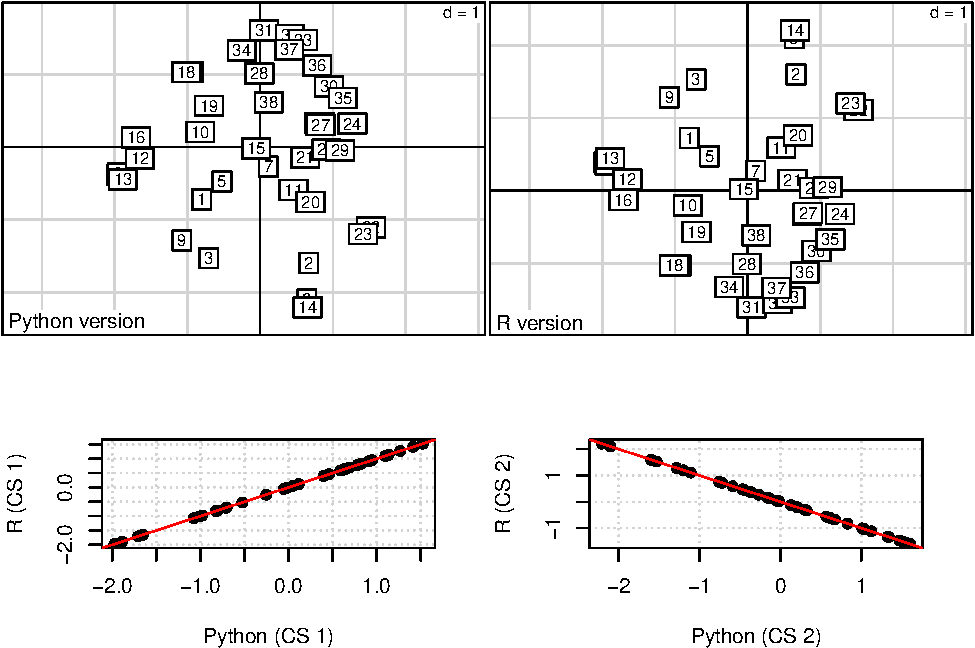
\includegraphics[keepaspectratio]{RandPytonAnalysisPDF_files/RandPytonAnalysisPDF_files/figure-latex/unnamed-chunk-37-1.pdf}}

\begin{Shaded}
\begin{Highlighting}[]
\NormalTok{par(mfrow=c(2,2))}
\NormalTok{plot(py$X[,1],acm1$tab[,1],panel.first=c(grid()),xlab="Python (col 1 of Z)",}
\NormalTok{     ylab="R (col 1 of tab)",pch=19);abline(0,1,col="red")}
\NormalTok{plot(py$ted$c1[,1],acm1$c1[,1],panel.first=c(grid()),xlab="Python (normed Axis 1)",}
\NormalTok{     ylab="R (normed Axis 1)",pch=19);abline(0,1,col="red")}
\NormalTok{plot(py$ted$co[,1],acm1$co[,1],panel.first=c(grid()),xlab="Python (Axis 1)",}
\NormalTok{     ylab="R (Axis 1)",pch=19);abline(0,1,col="red")}
\end{Highlighting}
\end{Shaded}

\pandocbounded{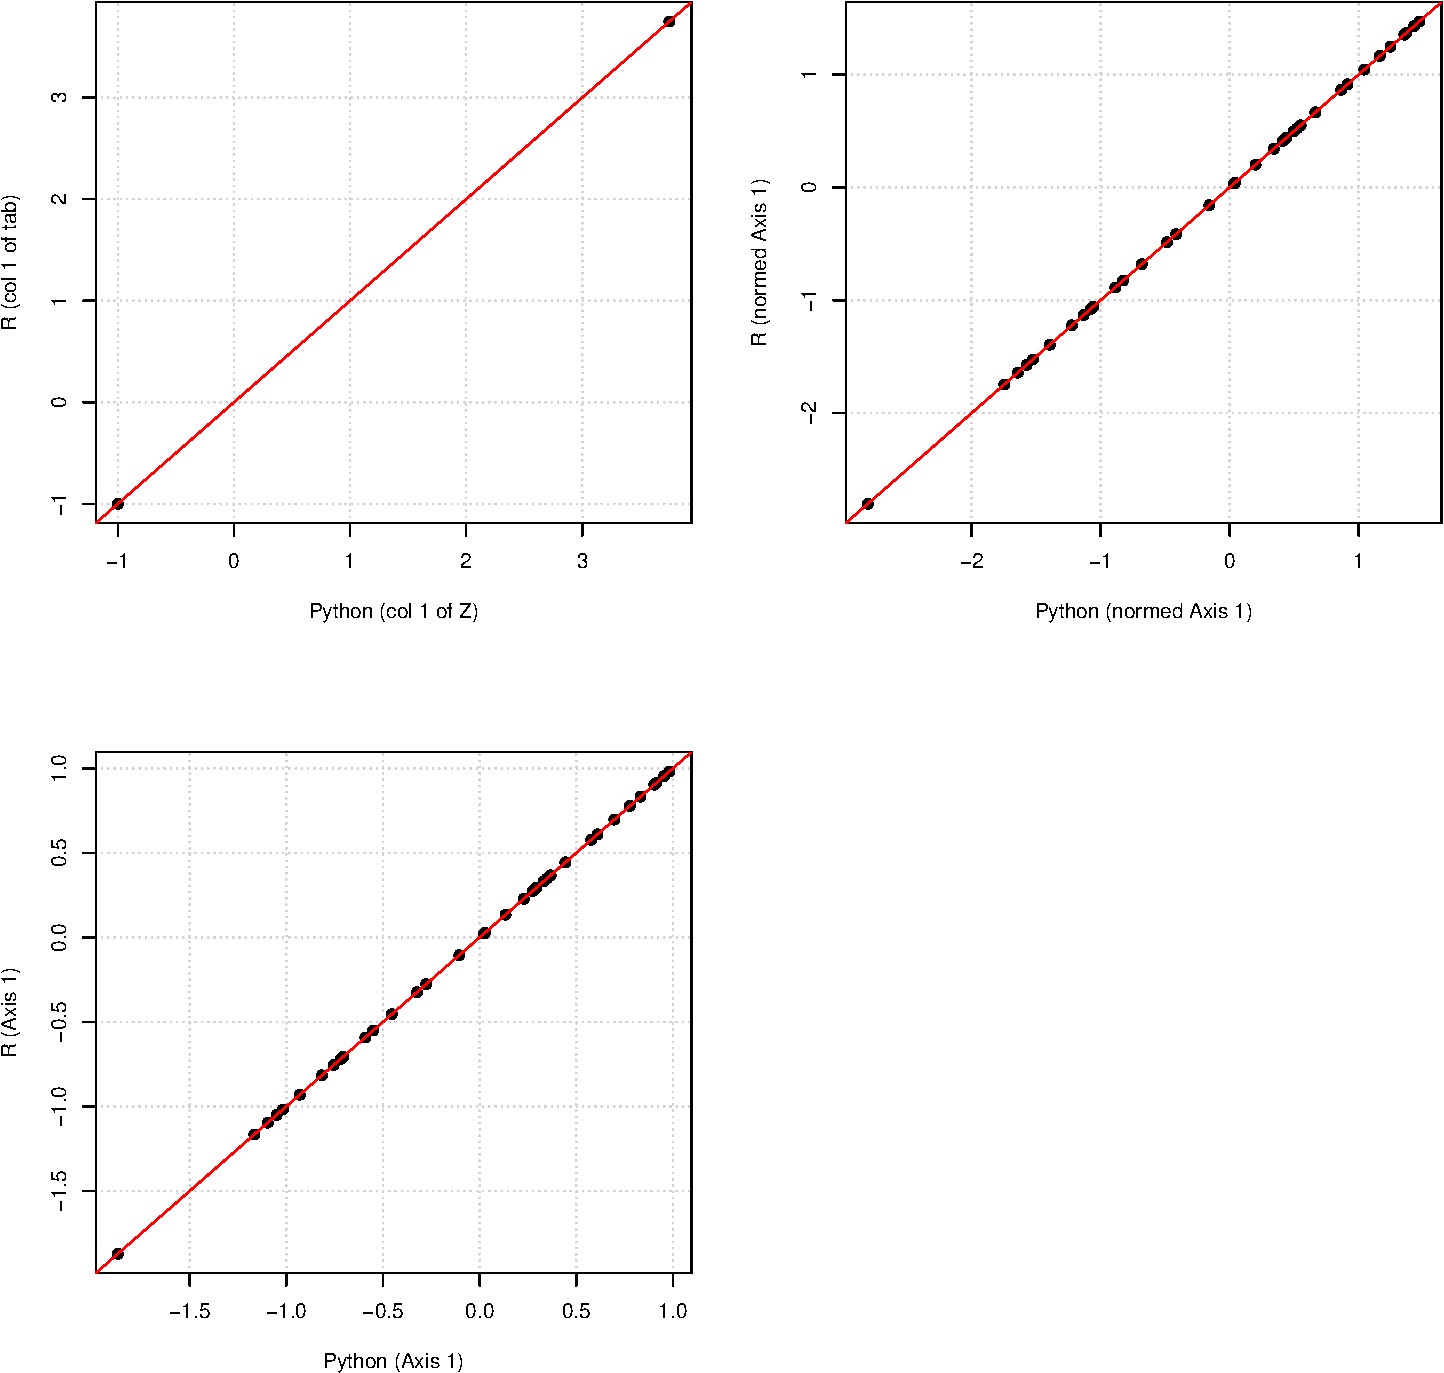
\includegraphics[keepaspectratio]{RandPytonAnalysisPDF_files/RandPytonAnalysisPDF_files/figure-latex/unnamed-chunk-38-1.pdf}}

\section{Class and object dudi}\label{class-and-object-dudi}

define the structure of the object and description of the elements based
on object `dudi' from R package ade4 (and ADE-4):

\begin{itemize}
\tightlist
\item
  tab
\item
  eig
\item
  rank
\item
  c1
\item
  co
\item
  l1
\item
  li
\end{itemize}

heritage for the PCA and COA (and other methods):

\begin{itemize}
\tightlist
\item
  tab
\item
  lw
\item
  cw
\item
  dudi
\item
  and specific elements
\end{itemize}

\subsection{\texorpdfstring{Object
\textbf{Dudi}}{Object Dudi}}\label{object-dudi}

\begin{Shaded}
\begin{Highlighting}[]
\NormalTok{class Dudi:}
\NormalTok{  def \_\_init\_\_(self,tab,cw,lw,eig,rank,nf,c1,co,l1,li):}
\NormalTok{    self.tab = tab}
\NormalTok{    self.cw = cw}
\NormalTok{    self.lw = lw}
\NormalTok{    self.eig = eig}
\NormalTok{    self.rank = rank}
\NormalTok{    self.nf = nf}
\NormalTok{    self.c1 = c1}
\NormalTok{    self.co = co}
\NormalTok{    self.l1 = l1}
\NormalTok{    self.li = li}

\NormalTok{def pyDudi(X,cw,lw,nf):}
\NormalTok{  dim = X.shape}
\NormalTok{  n = dim[0]}
\NormalTok{  p = dim[1]}
\NormalTok{  nf0 = nf{-}1}
\NormalTok{  \# n=len(X)}
\NormalTok{  \# p=len(X.columns)}
\NormalTok{  D = np.diag(np.sqrt(lw))}
\NormalTok{  Q = np.diag(np.sqrt(cw))}
  
\NormalTok{  \# XtDXQ =\textgreater{} problem  with Q !!!}
\NormalTok{  XD = np.dot(X.T,D).T}
\NormalTok{  XD = np.dot(XD,Q)}
\NormalTok{  XtX = np.dot(XD.T,XD)}
  
\NormalTok{  \# decomposition}
\NormalTok{  eigenvalues, eigenvectors = np.linalg.eig(XtX)}
\NormalTok{  index = np.argsort(eigenvalues)[::{-}1]}
  
\NormalTok{  \# np.nonzero(eigenvalues)[0]}
\NormalTok{  eigenvalues = eigenvalues.real}
\NormalTok{  eigenvectors = eigenvectors.real}
\NormalTok{  eigenvalues=eigenvalues[index]}
\NormalTok{  eigenvectors=eigenvectors[:,index]}
\NormalTok{  \# results}
\NormalTok{  rank = len(np.nonzero(eigenvalues)[0])}
\NormalTok{  C1 = np.dot(np.diag(1/np.sqrt(cw)),eigenvectors[:,0:nf])}
\NormalTok{  \#C1 = eigenvectors[:,0:nf]}
\NormalTok{  XQ = np.dot(X,np.diag(cw))}
\NormalTok{  Li = np.dot(XQ, C1)}
  
\NormalTok{  \# need to adjust the weighting (problem with sqrt)}
\NormalTok{  L1 = np.dot(Li,np.diag(1/np.sqrt(eigenvalues[0:nf])))}
\NormalTok{  Co = np.dot(C1,np.diag(np.sqrt(eigenvalues[0:nf])))}
\NormalTok{  return Dudi(X,cw,lw,eigenvalues,rank,nf,C1,Co,L1,Li);}
\end{Highlighting}
\end{Shaded}

\subsection{test pour PCA}\label{test-pour-pca}

\begin{Shaded}
\begin{Highlighting}[]
\NormalTok{def pyPCA(X,cw=None,lw=None,nf=2,center=True,scale=True):}
\NormalTok{  dim = X.shape}
\NormalTok{  n = dim[0]}
\NormalTok{  p = dim[1]  }
\NormalTok{  if center:}
\NormalTok{    X = X{-}X.mean()}
\NormalTok{  if scale:}
\NormalTok{    X = X/X.std(ddof=0)}
\NormalTok{  if lw==None :}
\NormalTok{    lw = pd.DataFrame(np.repeat(1/n,n))[0]}
\NormalTok{  if cw==None :}
\NormalTok{    cw = pd.DataFrame(np.repeat(1,p))[0]}
\NormalTok{  dudi = pyDudi(X,cw,lw,nf)  }
\NormalTok{  return dudi;}
\end{Highlighting}
\end{Shaded}

\begin{Shaded}
\begin{Highlighting}[]
\NormalTok{pca1 = pyPCA(deugtab)}
\end{Highlighting}
\end{Shaded}

\subsection{test pour COA}\label{test-pour-coa}

\begin{Shaded}
\begin{Highlighting}[]
\NormalTok{def pyCOA(X,nf=2):}
\NormalTok{  sumX = X.sum().sum()}
\NormalTok{  sumCol =  X.sum(axis=0)}
\NormalTok{  sumRow = X.sum(axis=1)}
\NormalTok{  pij = X/sumX}
\NormalTok{  pi = sumRow/sumX}
\NormalTok{  pj = sumCol/sumX}
\NormalTok{  Dj = np.diag(1/pj)}
\NormalTok{  Di = np.diag(1/pi)}
\NormalTok{  Z = np.dot(Di,pij)}
\NormalTok{  Z = np.dot(Z,Dj)}
\NormalTok{  Z = Z {-} 1}
\NormalTok{  Z = np.nan\_to\_num(Z)}
\NormalTok{  dudi = pyDudi(Z,pj,pi,nf)  }
\NormalTok{  return dudi;}
\end{Highlighting}
\end{Shaded}

\begin{Shaded}
\begin{Highlighting}[]
\NormalTok{coa1 = pyCOA(fau)}
\end{Highlighting}
\end{Shaded}

\subsection{test pour ACM}\label{test-pour-acm}

\begin{Shaded}
\begin{Highlighting}[]
\NormalTok{def disjonctif(X):}
\NormalTok{  X\_cat = X.astype("category")}
\NormalTok{  X\_dis = pd.get\_dummies(X\_cat)}
\NormalTok{  X\_dis = X\_dis*1}
\NormalTok{  return X\_dis;}

\NormalTok{def pyACM(X,lw=None,nf=2):}
\NormalTok{  Xdis = disjonctif(ours)}
\NormalTok{  m = Xdis.shape[1]}
\NormalTok{  n = Xdis.shape[0]}
\NormalTok{  v = ours.shape[1]}
\NormalTok{  if lw==None :}
\NormalTok{    lw = pd.DataFrame(np.repeat(1/n,n))[0]}
\NormalTok{  D = np.diag(lw)}
\NormalTok{  cw = np.dot(np.dot(Xdis.T,D), np.ones(n)) }
\NormalTok{  Dm = np.diag(cw)}
\NormalTok{  X = np.dot(Xdis,np.diag(1/cw)){-}1}
\NormalTok{  cw = cw/v}
\NormalTok{  dudi = pyDudi(X,cw,lw,nf)    }
\NormalTok{  return dudi;}
\end{Highlighting}
\end{Shaded}

\begin{Shaded}
\begin{Highlighting}[]
\NormalTok{mca1 = pyACM(ours)}
\end{Highlighting}
\end{Shaded}

\section{Generate Python package called
pydudi}\label{generate-python-package-called-pydudi}

construction of the file called `setup.py' in the folder

\begin{verbatim}
from setuptools import setup, find_packages
setup(
    name='pydudi',
    version='1.0',
    packages=find_packages(),
    description='Implementation Test of the duality diagram based on ade4 works',
    author='Pierre Bady',
    author_email='pierre.bady@gmail.com',
    install_requires=[],
)
\end{verbatim}

contruction of the file ``\textbf{init}.py'' in the subfolder

\begin{verbatim}
__all__ = ["Ktab","pyACM","pyCOA","pyDudi","pyPCA"]
\end{verbatim}

constrcution nof the archive (deprecated!!!)

\begin{verbatim}
python setup.py sdist bdist_wheel
\end{verbatim}

it's recommanded to use the following code (see:
\url{https://blog.stephane-robert.info/docs/developper/programmation/python/modules/})

\begin{verbatim}
pip install build twine
python -m build          # ou : uv build
twine upload dist/*      # authentification par jeton API PyPI
\end{verbatim}

\section{Construction of the function dudi in
Rcpp}\label{construction-of-the-function-dudi-in-rcpp}

\subsection{Test Rcpp: correlation between two
variables}\label{test-rcpp-correlation-between-two-variables}

\begin{Shaded}
\begin{Highlighting}[]
\NormalTok{require(parallel)}
\end{Highlighting}
\end{Shaded}

\begin{verbatim}
## Le chargement a nécessité le package : parallel
\end{verbatim}

\begin{Shaded}
\begin{Highlighting}[]
\NormalTok{require(Rcpp)}
\end{Highlighting}
\end{Shaded}

\begin{verbatim}
## Le chargement a nécessité le package : Rcpp
\end{verbatim}

\begin{Shaded}
\begin{Highlighting}[]
\NormalTok{require(RcppArmadillo)}
\end{Highlighting}
\end{Shaded}

\begin{verbatim}
## Le chargement a nécessité le package : RcppArmadillo
\end{verbatim}

\begin{Shaded}
\begin{Highlighting}[]
\NormalTok{\#Sys.setenv("PKG\_CXXFLAGS"="{-}fopenmp")}
\NormalTok{\#Sys.setenv("PKG\_LIBS"="{-}fopenmp")}
\NormalTok{sourceCpp(file.path(getwd(),"src","utility.cpp"))}
\end{Highlighting}
\end{Shaded}

correlation coefficient

\begin{Shaded}
\begin{Highlighting}[]
\NormalTok{cor(1:10, 2:11) }
\end{Highlighting}
\end{Shaded}

\begin{verbatim}
## [1] 1
\end{verbatim}

\begin{Shaded}
\begin{Highlighting}[]
\NormalTok{CORR(1:10, 2:11) }
\end{Highlighting}
\end{Shaded}

\begin{verbatim}
## [1] 1
\end{verbatim}

computation of the area under curve

\subsection{Object dudi}\label{object-dudi-1}

dudi obect with Rcpparmadillo

\begin{Shaded}
\begin{Highlighting}[]
\NormalTok{sourceCpp(file.path(getwd(),"src","utility.cpp"))}
\NormalTok{pca2 \textless{}{-} dudi.pca(deug$tab, center = TRUE, scale = TRUE, scan = FALSE)}
\NormalTok{test \textless{}{-} arc\_dudi(as.matrix(pca2$tab),pca2$cw,pca2$lw,2)}
\NormalTok{test$eig}
\end{Highlighting}
\end{Shaded}

\begin{verbatim}
##            [,1]
##  [1,] 3.1013578
##  [2,] 1.3629834
##  [3,] 1.0323269
##  [4,] 0.9340533
##  [5,] 0.7397529
##  [6,] 0.5746693
##  [7,] 0.5325414
##  [8,] 0.4375395
##  [9,] 0.2847754
\end{verbatim}

\begin{Shaded}
\begin{Highlighting}[]
\NormalTok{pca2$eig}
\end{Highlighting}
\end{Shaded}

\begin{verbatim}
## [1] 3.1013578 1.3629834 1.0323269 0.9340533 0.7397529 0.5746693 0.5325414 0.4375395
## [9] 0.2847754
\end{verbatim}

\begin{Shaded}
\begin{Highlighting}[]
\NormalTok{coordli \textless{}{-} test$li}
\NormalTok{par(mfrow=c(2,2))}
\NormalTok{s.label(coordli,sub="RcppArmadillo version")}
\NormalTok{s.label(pca2$li,sub="R version")}
\NormalTok{plot(coordli[,1],pca2$li[,1],panel.first=c(grid()),xlab="RcppArmadillo (CS 1)",}
\NormalTok{     ylab="R (CS 1)",pch=19);abline(0,{-}1,col="red")}
\NormalTok{plot(coordli[,2],pca2$li[,2],panel.first=c(grid()),xlab="RcppArmadillo (CS 2)",}
\NormalTok{     ylab="R (CS 2)",pch=19);abline(0,{-}1,col="red")}
\end{Highlighting}
\end{Shaded}

\pandocbounded{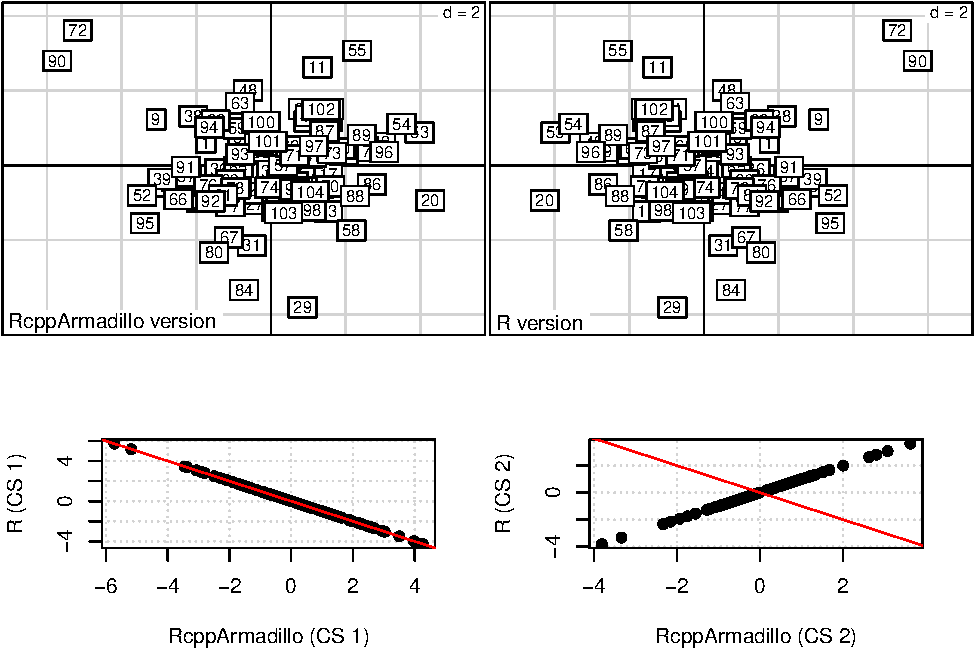
\includegraphics[keepaspectratio]{RandPytonAnalysisPDF_files/RandPytonAnalysisPDF_files/figure-latex/unnamed-chunk-50-1.pdf}}

\begin{Shaded}
\begin{Highlighting}[]
\NormalTok{coordl1 \textless{}{-} test$l1}
\NormalTok{par(mfrow=c(2,2))}
\NormalTok{s.label(coordl1,sub="RcppArmadillo version")}
\NormalTok{s.label(pca2$l1,sub="R version")}
\NormalTok{plot(coordl1[,1],pca2$l1[,1],panel.first=c(grid()),xlab="RcppArmadillo (CS 1)",}
\NormalTok{     ylab="R (CS 1)",pch=19);abline(0,{-}1,col="red")}
\NormalTok{plot(coordl1[,2],pca2$l1[,2],panel.first=c(grid()),xlab="RcppArmadillo (CS 2)",}
\NormalTok{     ylab="R (CS 2)",pch=19);abline(0,{-}1,col="red")}
\end{Highlighting}
\end{Shaded}

\pandocbounded{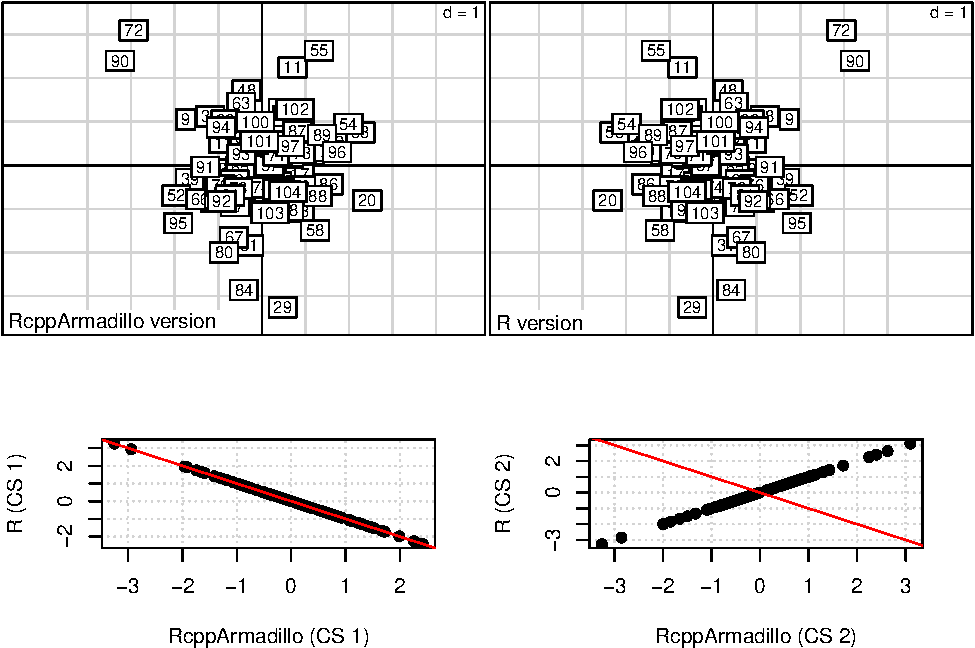
\includegraphics[keepaspectratio]{RandPytonAnalysisPDF_files/RandPytonAnalysisPDF_files/figure-latex/unnamed-chunk-51-1.pdf}}

\begin{Shaded}
\begin{Highlighting}[]
\NormalTok{par(mfrow=c(2,2))}
\NormalTok{s.corcircle(test$co,sub="RcppArmadillo version")}
\NormalTok{s.corcircle(pca2$co,sub="R version")}
\NormalTok{plot(test$c1[,1],pca2$c1[,1],panel.first=c(grid()),xlab="RcppArmadillo (axis 1)",}
\NormalTok{     ylab="R (axis 1)",pch=19);abline(0,{-}1,col="red")}
\NormalTok{plot(test$c1[,2],pca2$c1[,2],panel.first=c(grid()),xlab="RcppArmadillo (axis 2)",}
\NormalTok{     ylab="R (axis 2)",pch=19);abline(0,{-}1,col="red")}
\end{Highlighting}
\end{Shaded}

\pandocbounded{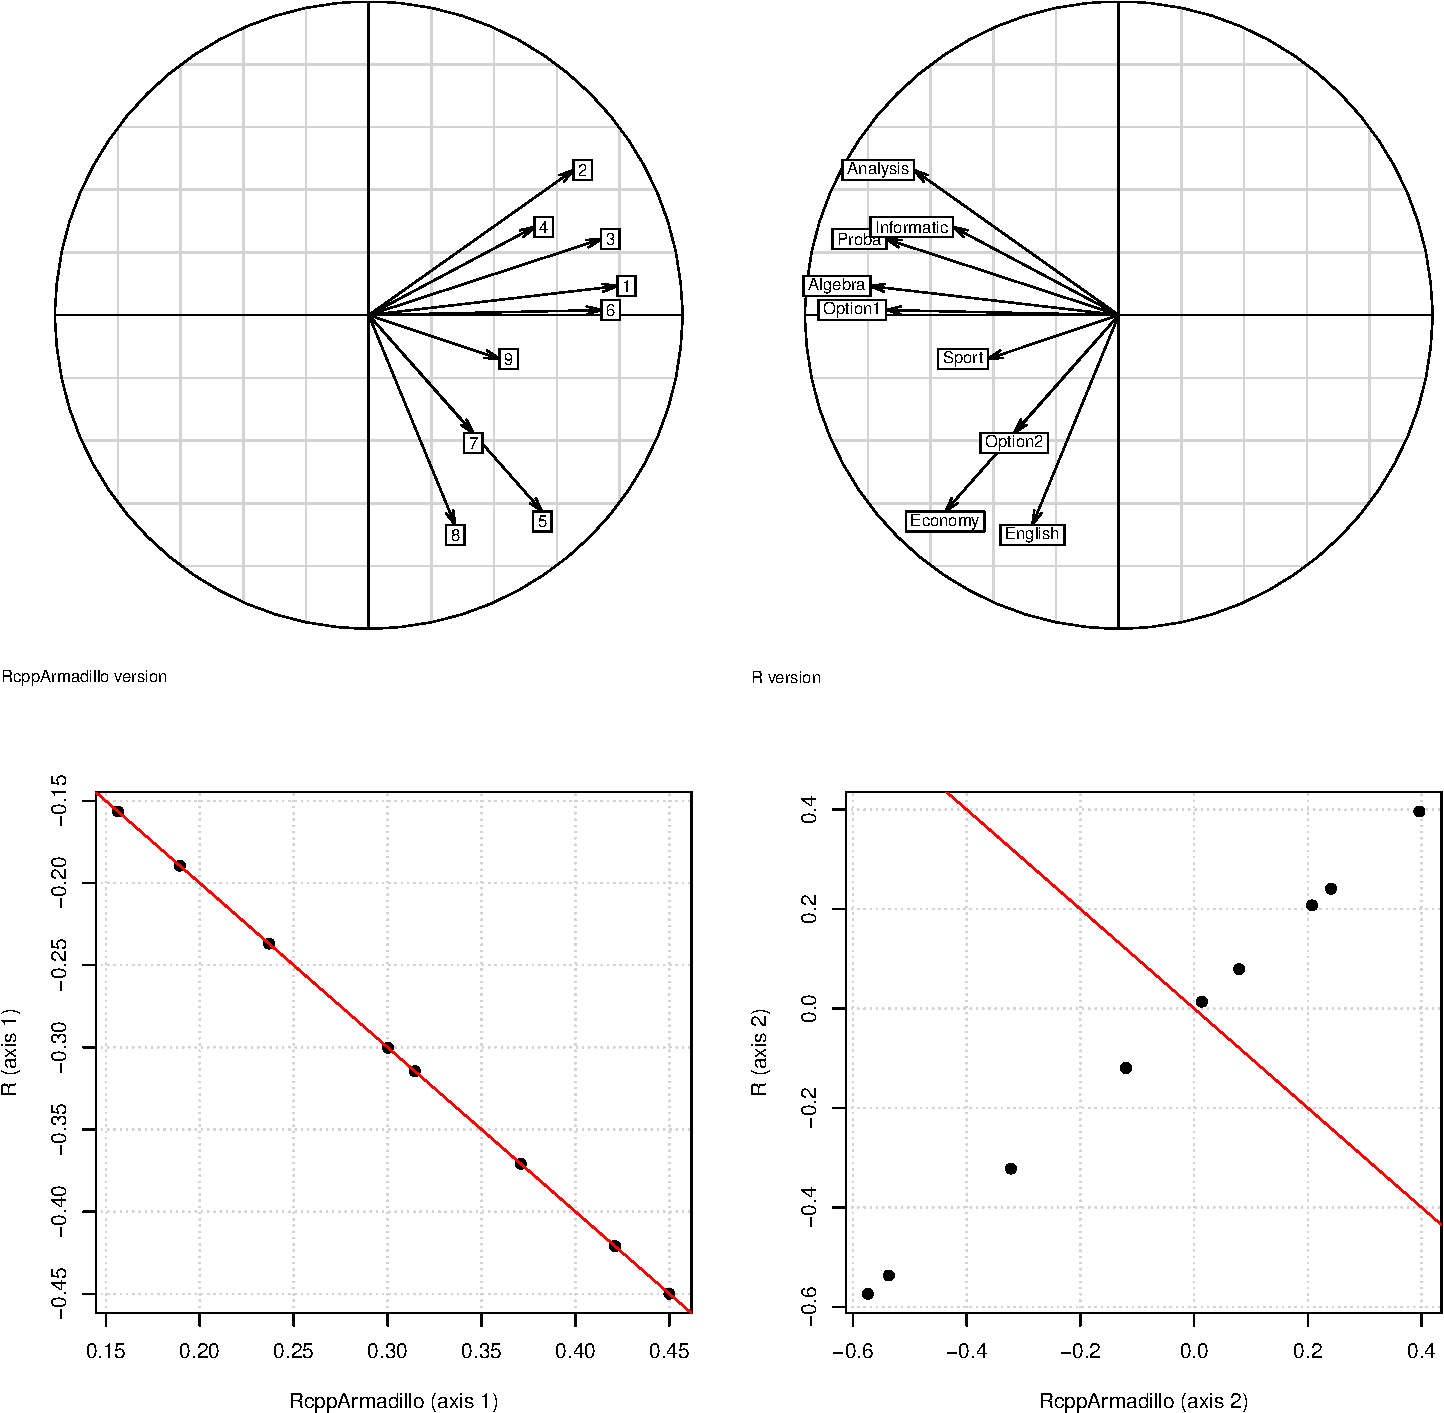
\includegraphics[keepaspectratio]{RandPytonAnalysisPDF_files/RandPytonAnalysisPDF_files/figure-latex/unnamed-chunk-52-1.pdf}}

\subsection{Test PCA}\label{test-pca}

argument for the function cpca:

\begin{itemize}
\tightlist
\item
  X: matrix
\item
  cw: numeric vector corresponding to the column weighting
\item
  lw: numeric vector corresponding to the row weighting
\item
  nf: number of selected axes
\item
  center: 1 for TRUE, 0 for FALSE
\item
  scale: 1 for TRUE, 0 for FALSE
\end{itemize}

\begin{Shaded}
\begin{Highlighting}[]
\NormalTok{sourceCpp(file.path(getwd(),"src","utility.cpp"))}
\NormalTok{test2 \textless{}{-} arc\_pca(as.matrix(deug$tab),pca2$cw,pca2$lw,2,1,1)}
\NormalTok{pca2$eig}
\end{Highlighting}
\end{Shaded}

\begin{verbatim}
## [1] 3.1013578 1.3629834 1.0323269 0.9340533 0.7397529 0.5746693 0.5325414 0.4375395
## [9] 0.2847754
\end{verbatim}

\begin{Shaded}
\begin{Highlighting}[]
\NormalTok{test2$eig}
\end{Highlighting}
\end{Shaded}

\begin{verbatim}
##            [,1]
##  [1,] 3.1013578
##  [2,] 1.3629834
##  [3,] 1.0323269
##  [4,] 0.9340533
##  [5,] 0.7397529
##  [6,] 0.5746693
##  [7,] 0.5325414
##  [8,] 0.4375395
##  [9,] 0.2847754
\end{verbatim}

\begin{Shaded}
\begin{Highlighting}[]
\NormalTok{coordli \textless{}{-} test2$li}
\NormalTok{par(mfrow=c(2,2))}
\NormalTok{s.label(coordli,sub="RcppArmadillo version")}
\NormalTok{s.label(pca2$li,sub="R version")}
\NormalTok{plot(coordli[,1],pca2$li[,1],panel.first=c(grid()),xlab="RcppArmadillo (CS 1)",}
\NormalTok{     ylab="R (CS 1)",pch=19);abline(0,{-}1,col="red")}
\NormalTok{plot(coordli[,2],pca2$li[,2],panel.first=c(grid()),xlab="RcppArmadillo (CS 2)",}
\NormalTok{     ylab="R (CS 2)",pch=19);abline(0,{-}1,col="red")}
\end{Highlighting}
\end{Shaded}

\pandocbounded{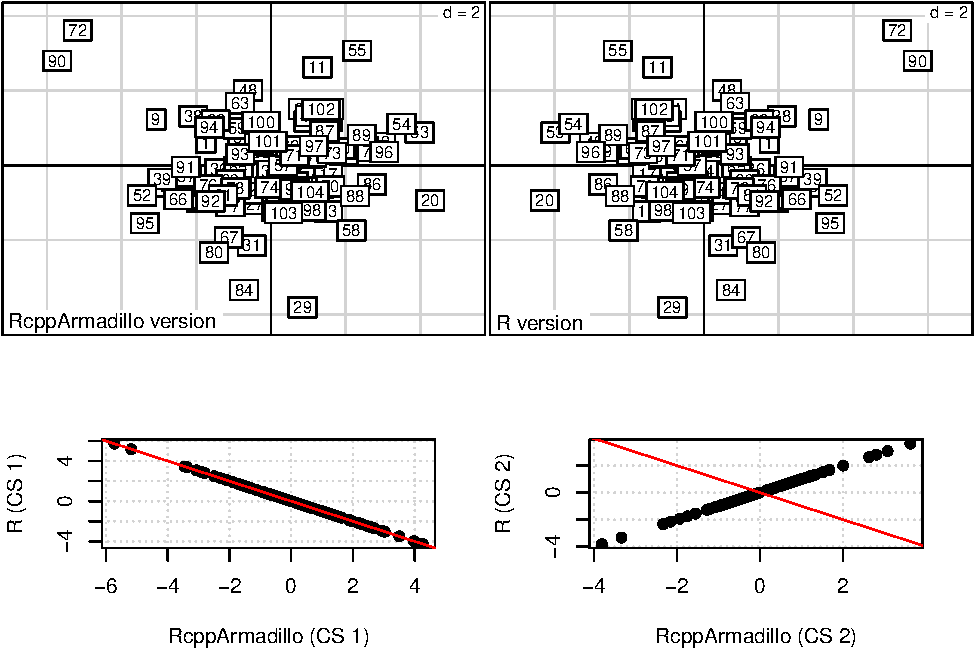
\includegraphics[keepaspectratio]{RandPytonAnalysisPDF_files/RandPytonAnalysisPDF_files/figure-latex/unnamed-chunk-54-1.pdf}}

\begin{Shaded}
\begin{Highlighting}[]
\NormalTok{coordl1 \textless{}{-} test2$l1}
\NormalTok{par(mfrow=c(2,2))}
\NormalTok{s.label(coordl1,sub="RcppArmadillo version")}
\NormalTok{s.label(pca2$l1,sub="R version")}
\NormalTok{plot(coordl1[,1],pca2$l1[,1],panel.first=c(grid()),xlab="RcppArmadillo (CS 1)",}
\NormalTok{     ylab="R (CS 1)",pch=19);abline(0,{-}1,col="red")}
\NormalTok{plot(coordl1[,2],pca2$l1[,2],panel.first=c(grid()),xlab="RcppArmadillo (CS 2)",}
\NormalTok{     ylab="R (CS 2)",pch=19);abline(0,{-}1,col="red")}
\end{Highlighting}
\end{Shaded}

\pandocbounded{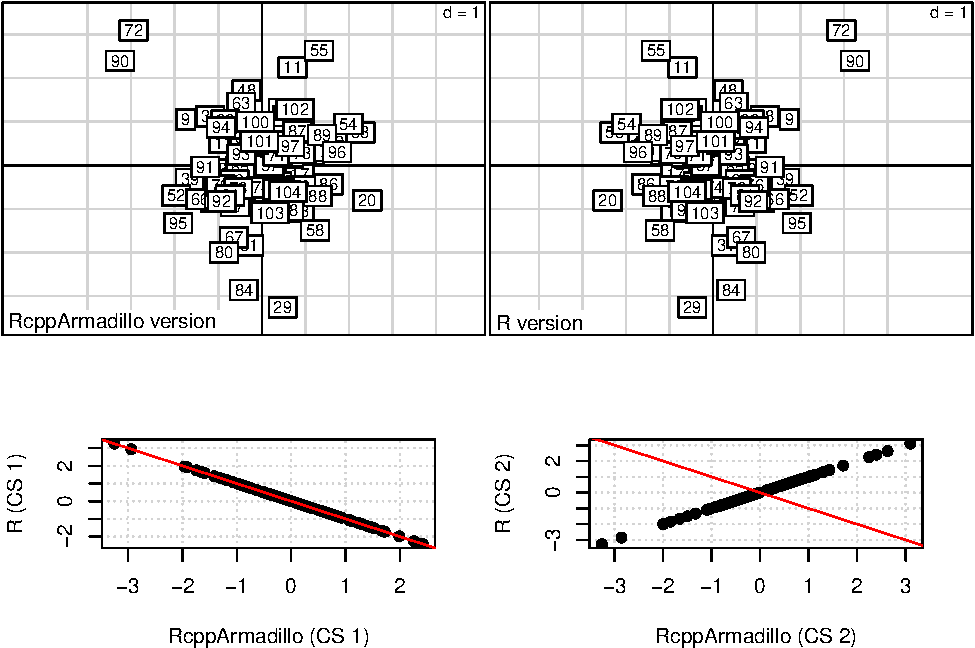
\includegraphics[keepaspectratio]{RandPytonAnalysisPDF_files/RandPytonAnalysisPDF_files/figure-latex/unnamed-chunk-55-1.pdf}}

\begin{Shaded}
\begin{Highlighting}[]
\NormalTok{par(mfrow=c(2,2))}
\NormalTok{s.corcircle(test2$co,sub="RcppArmadillo version")}
\NormalTok{s.corcircle(pca2$co,sub="R version")}
\NormalTok{plot(test2$c1[,1],pca2$c1[,1],panel.first=c(grid()),xlab="RcppArmadillo (axis 1)",}
\NormalTok{     ylab="R (axis 1)",pch=19);abline(0,{-}1,col="red")}
\NormalTok{plot(test2$c1[,2],pca2$c1[,2],panel.first=c(grid()),xlab="RcppArmadillo (axis 2)",}
\NormalTok{     ylab="R (axis 2)",pch=19);abline(0,{-}1,col="red")}
\end{Highlighting}
\end{Shaded}

\pandocbounded{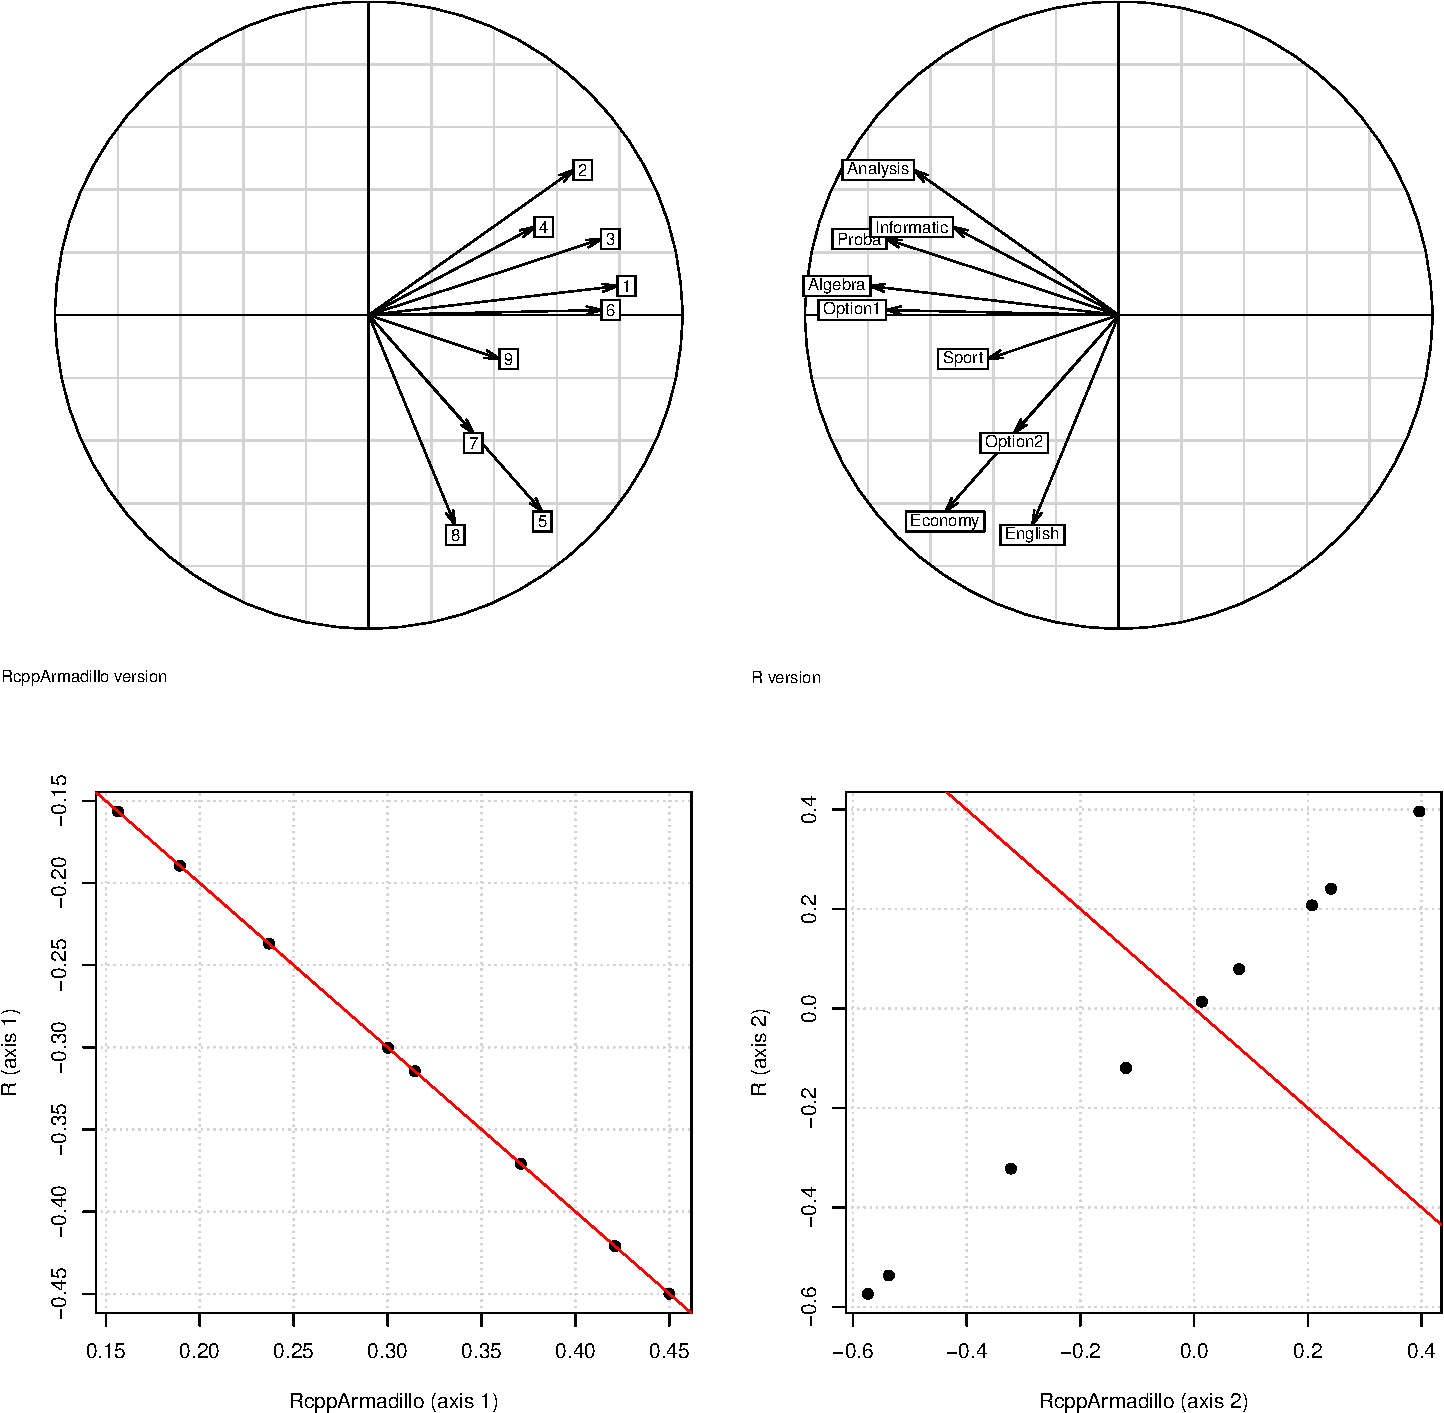
\includegraphics[keepaspectratio]{RandPytonAnalysisPDF_files/RandPytonAnalysisPDF_files/figure-latex/unnamed-chunk-56-1.pdf}}

\subsection{Test COA}\label{test-coa}

\begin{Shaded}
\begin{Highlighting}[]
\NormalTok{sourceCpp(file.path(getwd(),"src","utility.cpp"))}
\NormalTok{data(rpjdl)}
\NormalTok{chisq.test(rpjdl$fau)$statistic}
\end{Highlighting}
\end{Shaded}

\begin{verbatim}
## Warning in chisq.test(rpjdl$fau): L’approximation du Chi-2 est peut-être incorrecte
\end{verbatim}

\begin{verbatim}
## X-squared 
##  7323.597
\end{verbatim}

\begin{Shaded}
\begin{Highlighting}[]
\NormalTok{rpjdl.coa \textless{}{-} coa1 \textless{}{-} dudi.coa(rpjdl$fau, scannf = FALSE, nf = 4)}
\NormalTok{sum(rpjdl.coa$eig)*rpjdl.coa$N \# the same}
\end{Highlighting}
\end{Shaded}

\begin{verbatim}
## [1] 7323.597
\end{verbatim}

\begin{Shaded}
\begin{Highlighting}[]
\NormalTok{test \textless{}{-} arc\_coa(as.matrix(rpjdl$fau),nf=2)}
\end{Highlighting}
\end{Shaded}

\begin{Shaded}
\begin{Highlighting}[]
\NormalTok{coordli \textless{}{-} test$li}
\NormalTok{par(mfrow=c(2,2))}
\NormalTok{s.label(coordli,sub="Rcpp{-}Armadillo version")}
\NormalTok{s.label(coa1$li,sub="R version")}
\NormalTok{plot(coordli[,1],coa1$li[,1],panel.first=c(grid()),xlab="Rcpp{-}Armadillo (CS 1)",}
\NormalTok{     ylab="R (CS 1)",pch=19);abline(0,1,col="red")}
\NormalTok{plot(coordli[,2],coa1$li[,2],panel.first=c(grid()),xlab="Rcpp{-}Armadillo (CS 2)",}
\NormalTok{     ylab="R (CS 2)",pch=19);abline(0,{-}1,col="red")}
\end{Highlighting}
\end{Shaded}

\pandocbounded{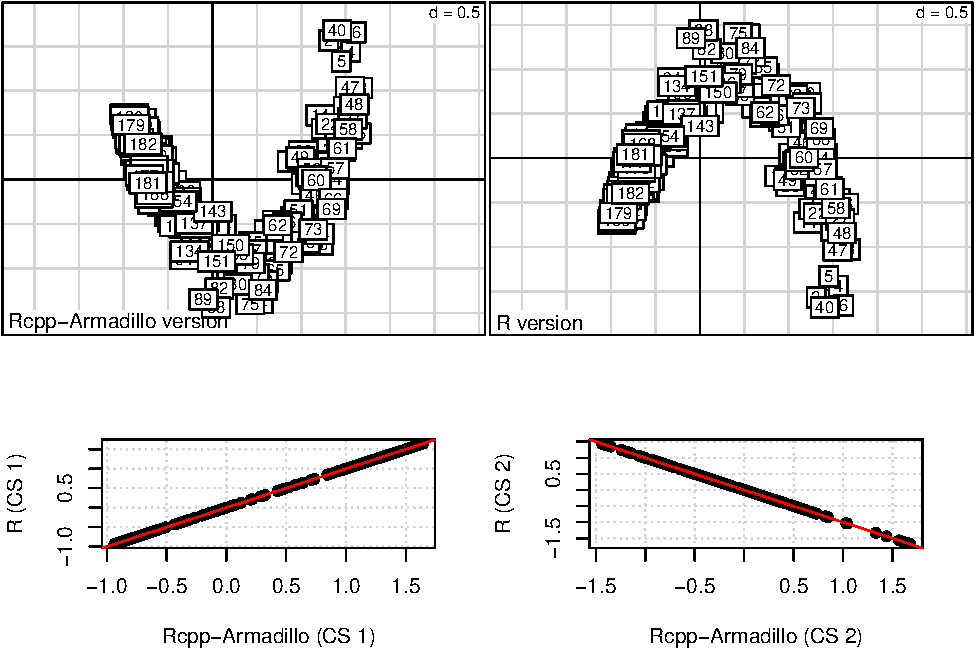
\includegraphics[keepaspectratio]{RandPytonAnalysisPDF_files/RandPytonAnalysisPDF_files/figure-latex/unnamed-chunk-58-1.pdf}}

\begin{Shaded}
\begin{Highlighting}[]
\NormalTok{coordl1 \textless{}{-} test$l1}
\NormalTok{par(mfrow=c(2,2))}
\NormalTok{s.label(coordl1,sub="Rcpp{-}Armadillo version")}
\NormalTok{s.label(coa1$l1,sub="R version")}
\NormalTok{plot(coordl1[,1],coa1$l1[,1],panel.first=c(grid()),xlab="Rcpp{-}Armadillo (CS 1)",}
\NormalTok{     ylab="R (CS 1)",pch=19);abline(0,1,col="red")}
\NormalTok{plot(coordl1[,2],coa1$l1[,2],panel.first=c(grid()),xlab="Rcpp{-}Armadillo (CS 2)",}
\NormalTok{     ylab="R (CS 2)",pch=19);abline(0,{-}1,col="red")}
\end{Highlighting}
\end{Shaded}

\pandocbounded{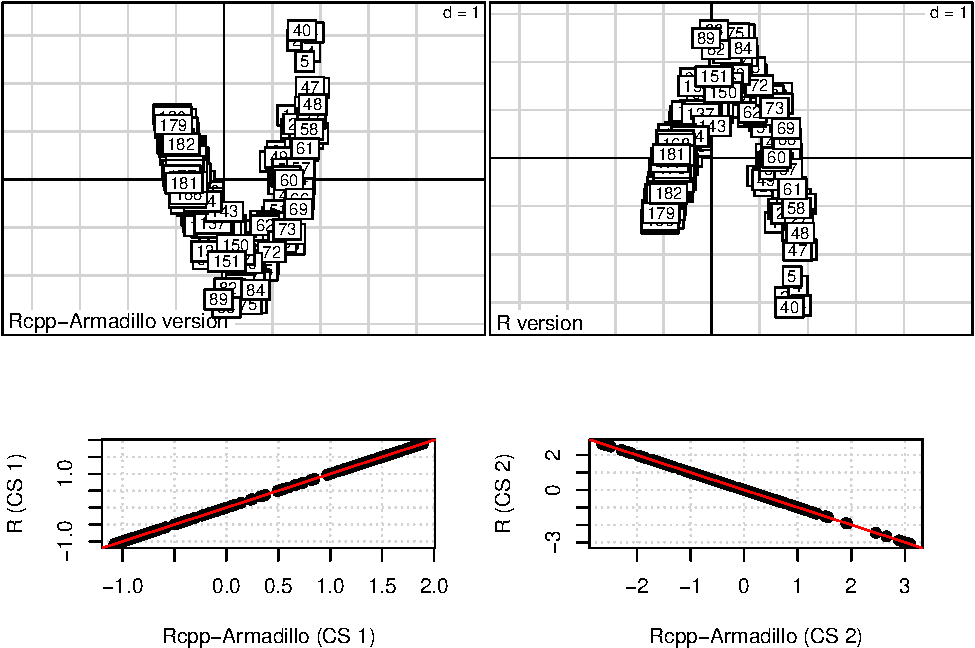
\includegraphics[keepaspectratio]{RandPytonAnalysisPDF_files/RandPytonAnalysisPDF_files/figure-latex/unnamed-chunk-59-1.pdf}}

\begin{Shaded}
\begin{Highlighting}[]
\NormalTok{par(mfrow=c(2,2))}
\NormalTok{plot(test$X[,1],coa1$tab[,1],panel.first=c(grid()),xlab="Rcpp{-}Armadillo (col 1 of Z)",}
\NormalTok{     ylab="R (col 1 of tab)",pch=19);abline(0,1,col="red")}
\NormalTok{plot(test$c1[,1],coa1$c1[,1],panel.first=c(grid()),xlab="Rcpp{-}Armadillo (normed Axis 1)",}
\NormalTok{     ylab="R (normed Axis 1)",pch=19);abline(0,1,col="red")}
\NormalTok{plot(test$co[,1],coa1$co[,1],panel.first=c(grid()),xlab="Rcpp{-}Armadillo (Axis 1)",}
\NormalTok{     ylab="R (Axis 1)",pch=19);abline(0,1,col="red")}
\end{Highlighting}
\end{Shaded}

\pandocbounded{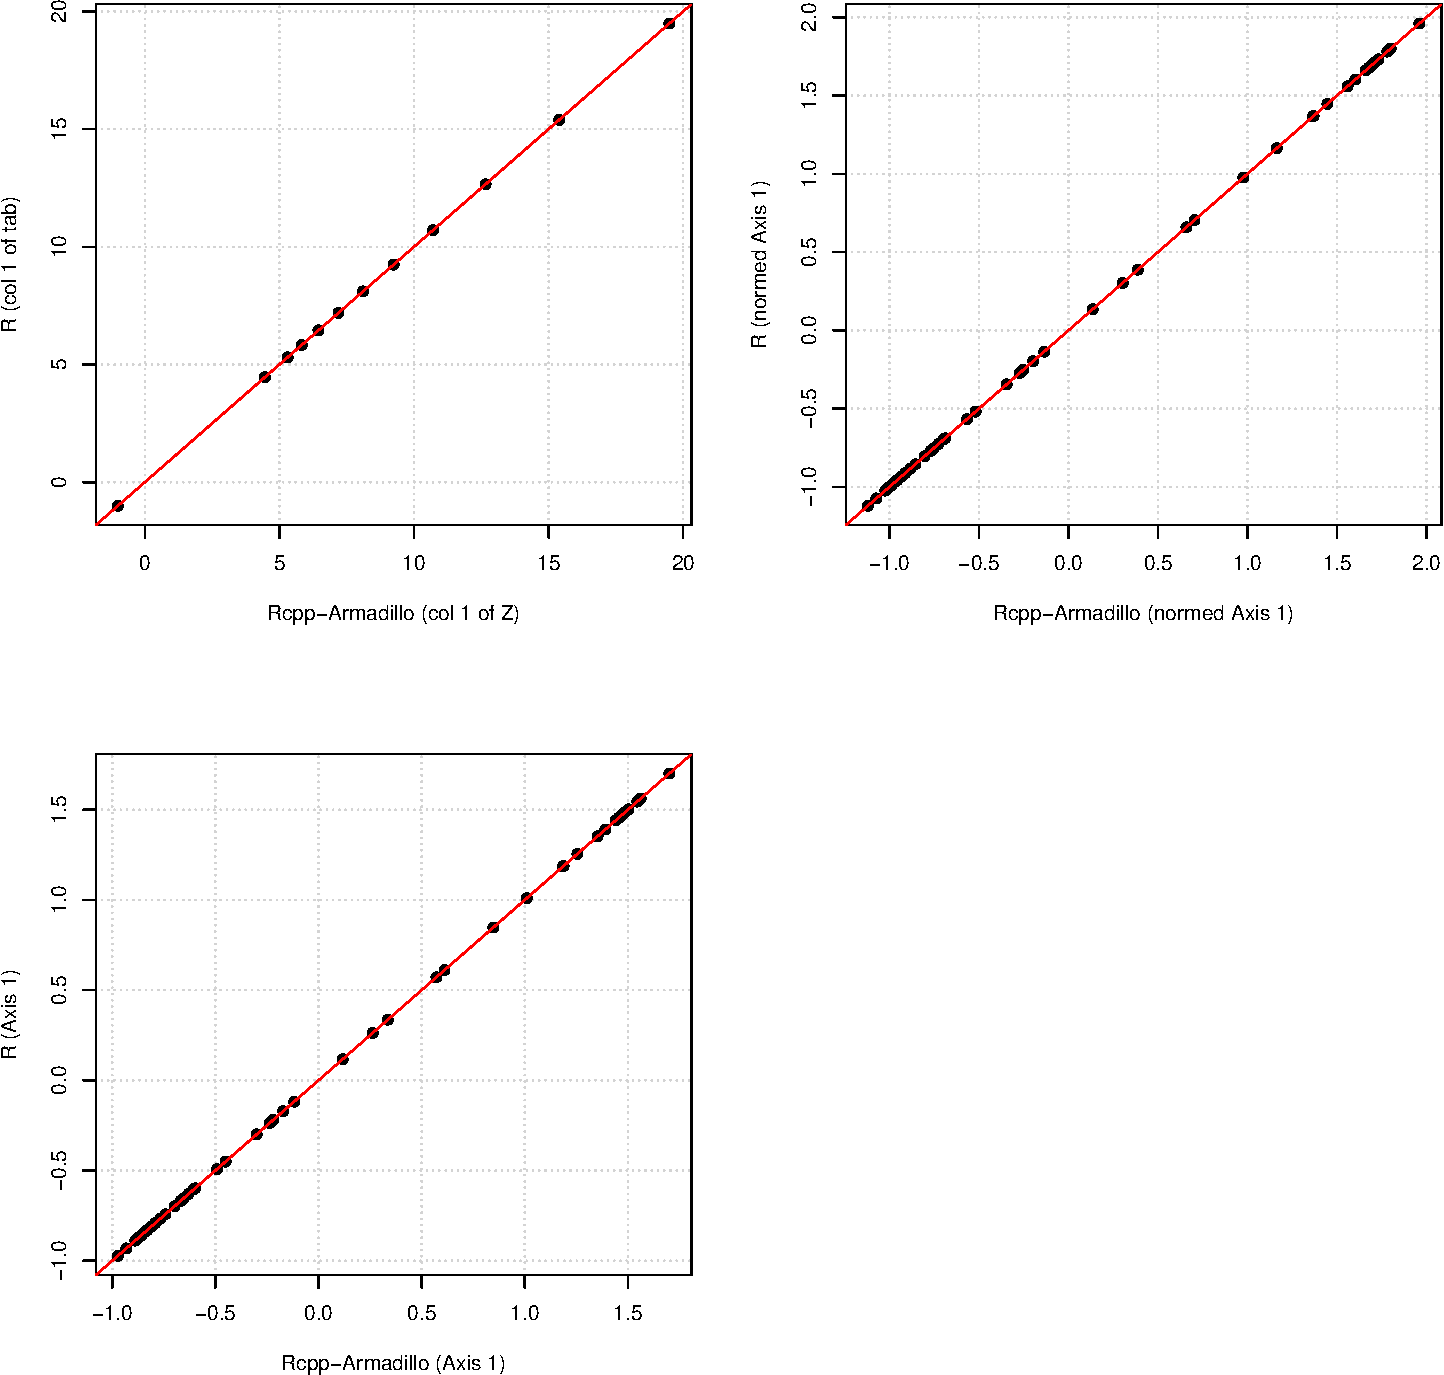
\includegraphics[keepaspectratio]{RandPytonAnalysisPDF_files/RandPytonAnalysisPDF_files/figure-latex/unnamed-chunk-60-1.pdf}}

\subsection{Test MCA}\label{test-mca}

\begin{Shaded}
\begin{Highlighting}[]
\NormalTok{data(ours)}
\NormalTok{summary(ours)}
\end{Highlighting}
\end{Shaded}

\begin{verbatim}
##  altit  deniv  cloiso domain boise  hetra  favor  inexp  citat  depart 
##  1: 8   1:13   1:12   1: 9   1:10   1:19   1:15   1:20   1:22   AHP:5  
##  2:17   2:14   2: 4   2:13   2:15   2: 5   2:12   2:10   2: 7   AM :4  
##  3:13   3:11   3:22   3:16   3:13   3:14   3:11   3: 8   3: 4   D  :5  
##                                                          4: 5   HP :8  
##                                                                 HS :4  
##                                                                 I  :5  
##                                                                 S  :7
\end{verbatim}

\begin{Shaded}
\begin{Highlighting}[]
\NormalTok{acm1 \textless{}{-} dudi.acm(ours, scan = FALSE)}
\end{Highlighting}
\end{Shaded}

for the first version of mca, we give the \textbf{disjonctif} table and
the variable number.

\begin{Shaded}
\begin{Highlighting}[]
\NormalTok{sourceCpp(file.path(getwd(),"src","utility.cpp"))}
\NormalTok{test \textless{}{-} arc\_mca\_proto(as.matrix(acm.disjonctif(ours)),lw=acm1$lw,v=ncol(ours),nf=2)}
\end{Highlighting}
\end{Shaded}

\begin{Shaded}
\begin{Highlighting}[]
\NormalTok{coordli \textless{}{-} test$li}
\NormalTok{par(mfrow=c(2,2))}
\NormalTok{s.label(coordli,sub="Rcpp{-}Armadillo version")}
\NormalTok{s.label(acm1$li,sub="R version")}
\NormalTok{plot(coordli[,1],acm1$li[,1],panel.first=c(grid()),xlab="Rcpp{-}Armadillo (CS 1)",}
\NormalTok{     ylab="R (CS 1)",pch=19);abline(0,{-}1,col="red")}
\NormalTok{plot(coordli[,2],acm1$li[,2],panel.first=c(grid()),xlab="Rcpp{-}Armadillo (CS 2)",}
\NormalTok{     ylab="R (CS 2)",pch=19);abline(0,1,col="red")}
\end{Highlighting}
\end{Shaded}

\pandocbounded{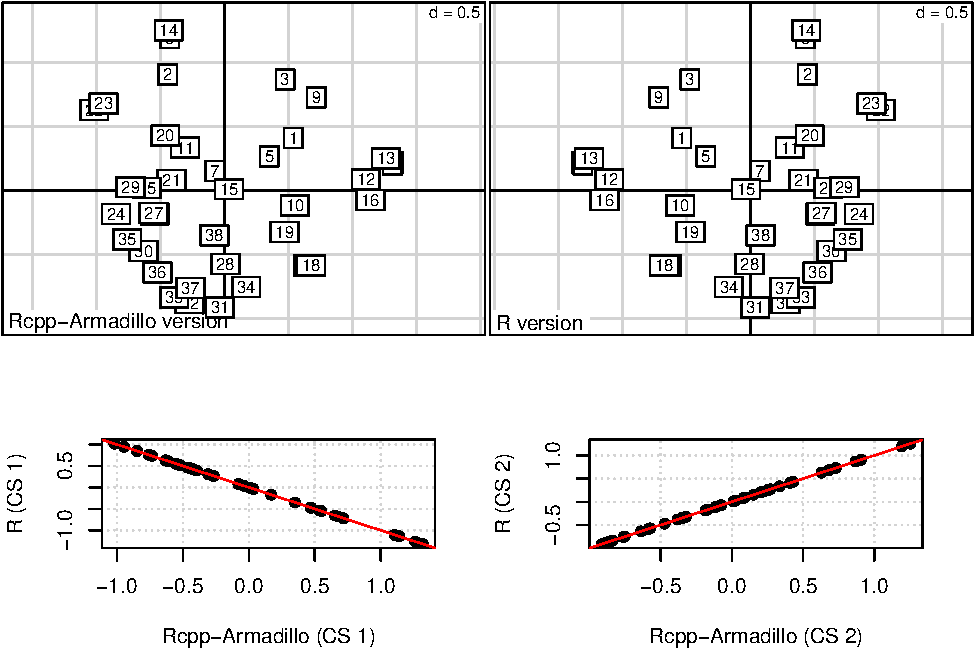
\includegraphics[keepaspectratio]{RandPytonAnalysisPDF_files/RandPytonAnalysisPDF_files/figure-latex/unnamed-chunk-63-1.pdf}}

\begin{Shaded}
\begin{Highlighting}[]
\NormalTok{coordl1 \textless{}{-} test$l1}
\NormalTok{par(mfrow=c(2,2))}
\NormalTok{s.label(coordl1,sub="Python version")}
\NormalTok{s.label(acm1$l1,sub="R version")}
\NormalTok{plot(coordl1[,1],acm1$l1[,1],panel.first=c(grid()),xlab="Rcpp{-}Armadillo (CS 1)",}
\NormalTok{     ylab="R (CS 1)",pch=19);abline(0,{-}1,col="red")}
\NormalTok{plot(coordl1[,2],acm1$l1[,2],panel.first=c(grid()),xlab="Rcpp{-}Armadillo (CS 2)",}
\NormalTok{     ylab="R (CS 2)",pch=19);abline(0,1,col="red")}
\end{Highlighting}
\end{Shaded}

\pandocbounded{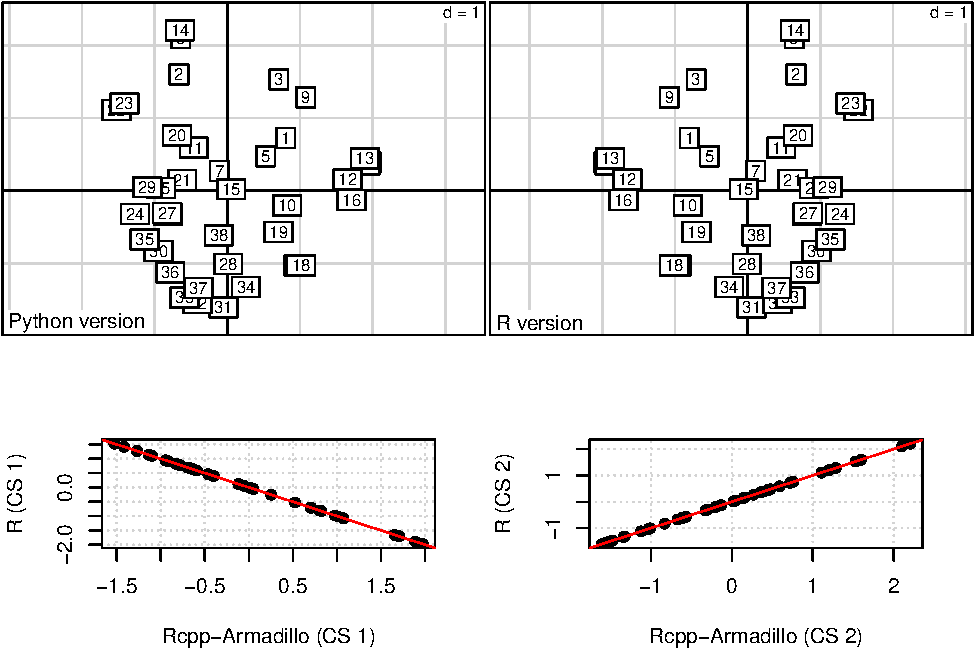
\includegraphics[keepaspectratio]{RandPytonAnalysisPDF_files/RandPytonAnalysisPDF_files/figure-latex/unnamed-chunk-64-1.pdf}}

\begin{Shaded}
\begin{Highlighting}[]
\NormalTok{par(mfrow=c(2,2))}
\NormalTok{plot(test$X[,1],acm1$tab[,1],panel.first=c(grid()),xlab="Rcpp{-}Armadillo (col 1 of Z)",}
\NormalTok{     ylab="R (col 1 of tab)",pch=19);abline(0,1,col="red")}
\NormalTok{plot(test$c1[,1],acm1$c1[,1],panel.first=c(grid()),xlab="Rcpp{-}Armadillo (normed Axis 1)",}
\NormalTok{     ylab="R (normed Axis 1)",pch=19);abline(0,{-}1,col="red")}
\NormalTok{plot(test$co[,1],acm1$co[,1],panel.first=c(grid()),xlab="Rcpp{-}Armadillo (Axis 1)",}
\NormalTok{     ylab="R (Axis 1)",pch=19);abline(0,{-}1,col="red")}
\end{Highlighting}
\end{Shaded}

\pandocbounded{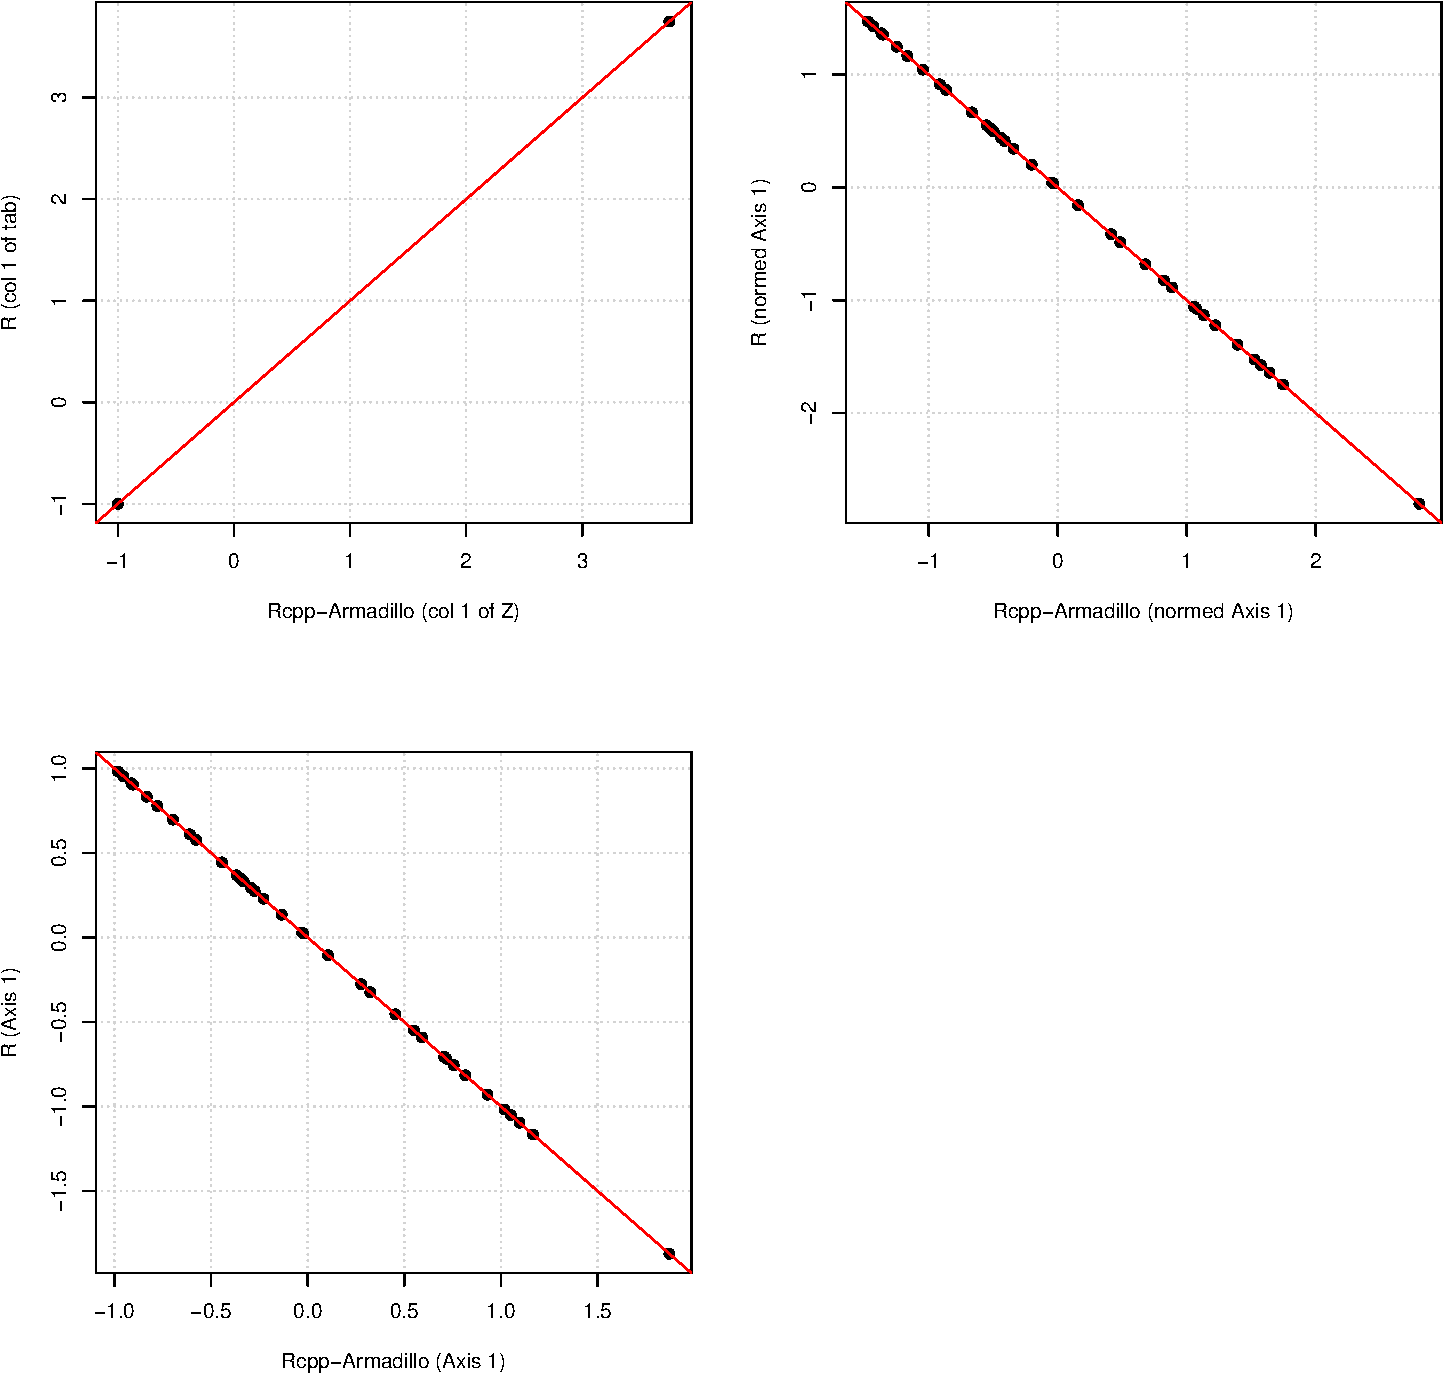
\includegraphics[keepaspectratio]{RandPytonAnalysisPDF_files/RandPytonAnalysisPDF_files/figure-latex/unnamed-chunk-65-1.pdf}}

encoding \textbf{disjonctif} table

\begin{Shaded}
\begin{Highlighting}[]
\NormalTok{sourceCpp(file.path(getwd(),"src","utility.cpp"))}
\NormalTok{w \textless{}{-} factor(c("a","a","b","c"))}
\NormalTok{acm.util(w)}
\end{Highlighting}
\end{Shaded}

\begin{verbatim}
##      a b c
## [1,] 1 0 0
## [2,] 1 0 0
## [3,] 0 1 0
## [4,] 0 0 1
\end{verbatim}

\begin{Shaded}
\begin{Highlighting}[]
\NormalTok{arc\_acmutil(w)}
\end{Highlighting}
\end{Shaded}

\begin{verbatim}
##      [,1] [,2] [,3]
## [1,]    1    0    0
## [2,]    1    0    0
## [3,]    0    1    0
## [4,]    0    0    1
\end{verbatim}

\begin{Shaded}
\begin{Highlighting}[]
\NormalTok{w1 \textless{}{-} factor(c("e","d","e","f"))}
\NormalTok{arc\_disjonctif(cbind(w,w1))}
\end{Highlighting}
\end{Shaded}

\begin{verbatim}
##      [,1] [,2] [,3] [,4] [,5] [,6]
## [1,]    1    0    0    0    1    0
## [2,]    1    0    0    1    0    0
## [3,]    0    1    0    0    1    0
## [4,]    0    0    1    0    0    1
\end{verbatim}

\begin{Shaded}
\begin{Highlighting}[]
\NormalTok{test \textless{}{-} arc\_mca( as.matrix(apply(ours,2,function(x) as.numeric(factor(x)))),}
\NormalTok{                 lw=acm1$lw,nf=2)}
\end{Highlighting}
\end{Shaded}

\begin{Shaded}
\begin{Highlighting}[]
\NormalTok{coordli \textless{}{-} test$li}
\NormalTok{par(mfrow=c(2,2))}
\NormalTok{s.label(coordli,sub="Rcpp{-}Armadillo version")}
\NormalTok{s.label(acm1$li,sub="R version")}
\NormalTok{plot(coordli[,1],acm1$li[,1],panel.first=c(grid()),xlab="Rcpp{-}Armadillo (CS 1)",}
\NormalTok{     ylab="R (CS 1)",pch=19);abline(0,{-}1,col="red")}
\NormalTok{plot(coordli[,2],acm1$li[,2],panel.first=c(grid()),xlab="Rcpp{-}Armadillo (CS 2)",}
\NormalTok{     ylab="R (CS 2)",pch=19);abline(0,1,col="red")}
\end{Highlighting}
\end{Shaded}

\pandocbounded{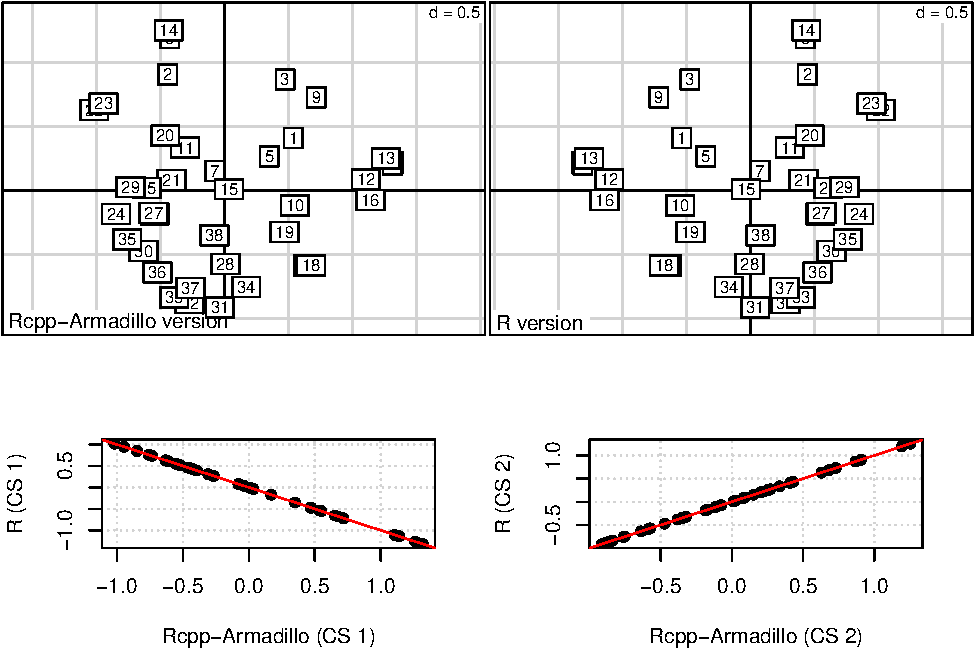
\includegraphics[keepaspectratio]{RandPytonAnalysisPDF_files/RandPytonAnalysisPDF_files/figure-latex/unnamed-chunk-68-1.pdf}}

\begin{Shaded}
\begin{Highlighting}[]
\NormalTok{coordl1 \textless{}{-} test$l1}
\NormalTok{par(mfrow=c(2,2))}
\NormalTok{s.label(coordl1,sub="Python version")}
\NormalTok{s.label(acm1$l1,sub="R version")}
\NormalTok{plot(coordl1[,1],acm1$l1[,1],panel.first=c(grid()),xlab="Rcpp{-}Armadillo (CS 1)",}
\NormalTok{     ylab="R (CS 1)",pch=19);abline(0,{-}1,col="red")}
\NormalTok{plot(coordl1[,2],acm1$l1[,2],panel.first=c(grid()),xlab="Rcpp{-}Armadillo (CS 2)",}
\NormalTok{     ylab="R (CS 2)",pch=19);abline(0,1,col="red")}
\end{Highlighting}
\end{Shaded}

\pandocbounded{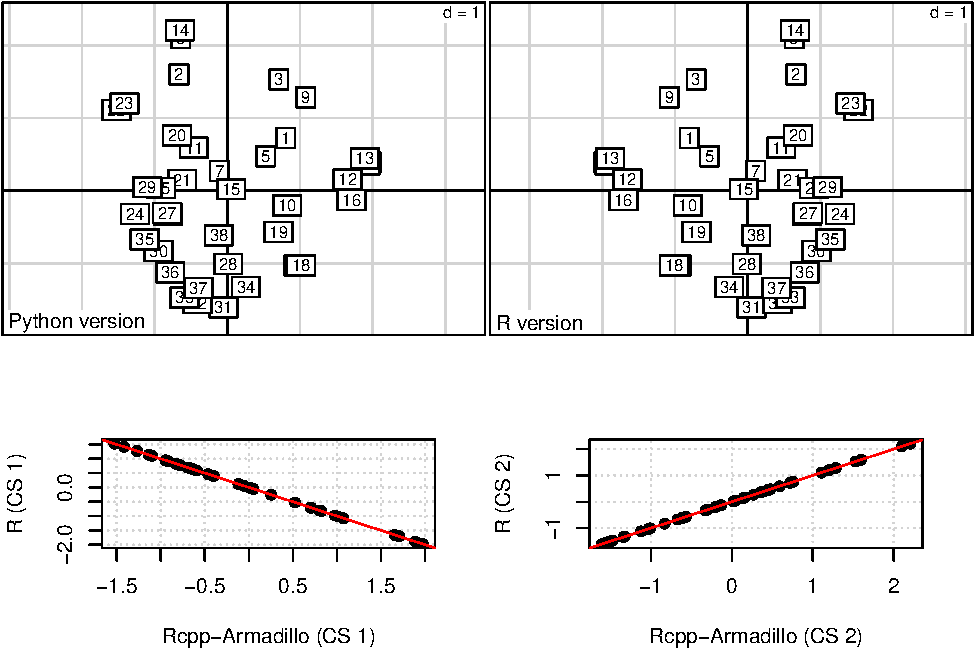
\includegraphics[keepaspectratio]{RandPytonAnalysisPDF_files/RandPytonAnalysisPDF_files/figure-latex/unnamed-chunk-69-1.pdf}}

\begin{Shaded}
\begin{Highlighting}[]
\NormalTok{par(mfrow=c(2,2))}
\NormalTok{plot(test$X[,1],acm1$tab[,1],panel.first=c(grid()),xlab="Rcpp{-}Armadillo (col 1 of Z)",}
\NormalTok{     ylab="R (col 1 of tab)",pch=19);abline(0,1,col="red")}
\NormalTok{plot(test$c1[,1],acm1$c1[,1],panel.first=c(grid()),xlab="Rcpp{-}Armadillo (normed Axis 1)",}
\NormalTok{     ylab="R (normed Axis 1)",pch=19);abline(0,{-}1,col="red")}
\NormalTok{plot(test$co[,1],acm1$co[,1],panel.first=c(grid()),xlab="Rcpp{-}Armadillo (Axis 1)",}
\NormalTok{     ylab="R (Axis 1)",pch=19);abline(0,{-}1,col="red")}
\end{Highlighting}
\end{Shaded}

\pandocbounded{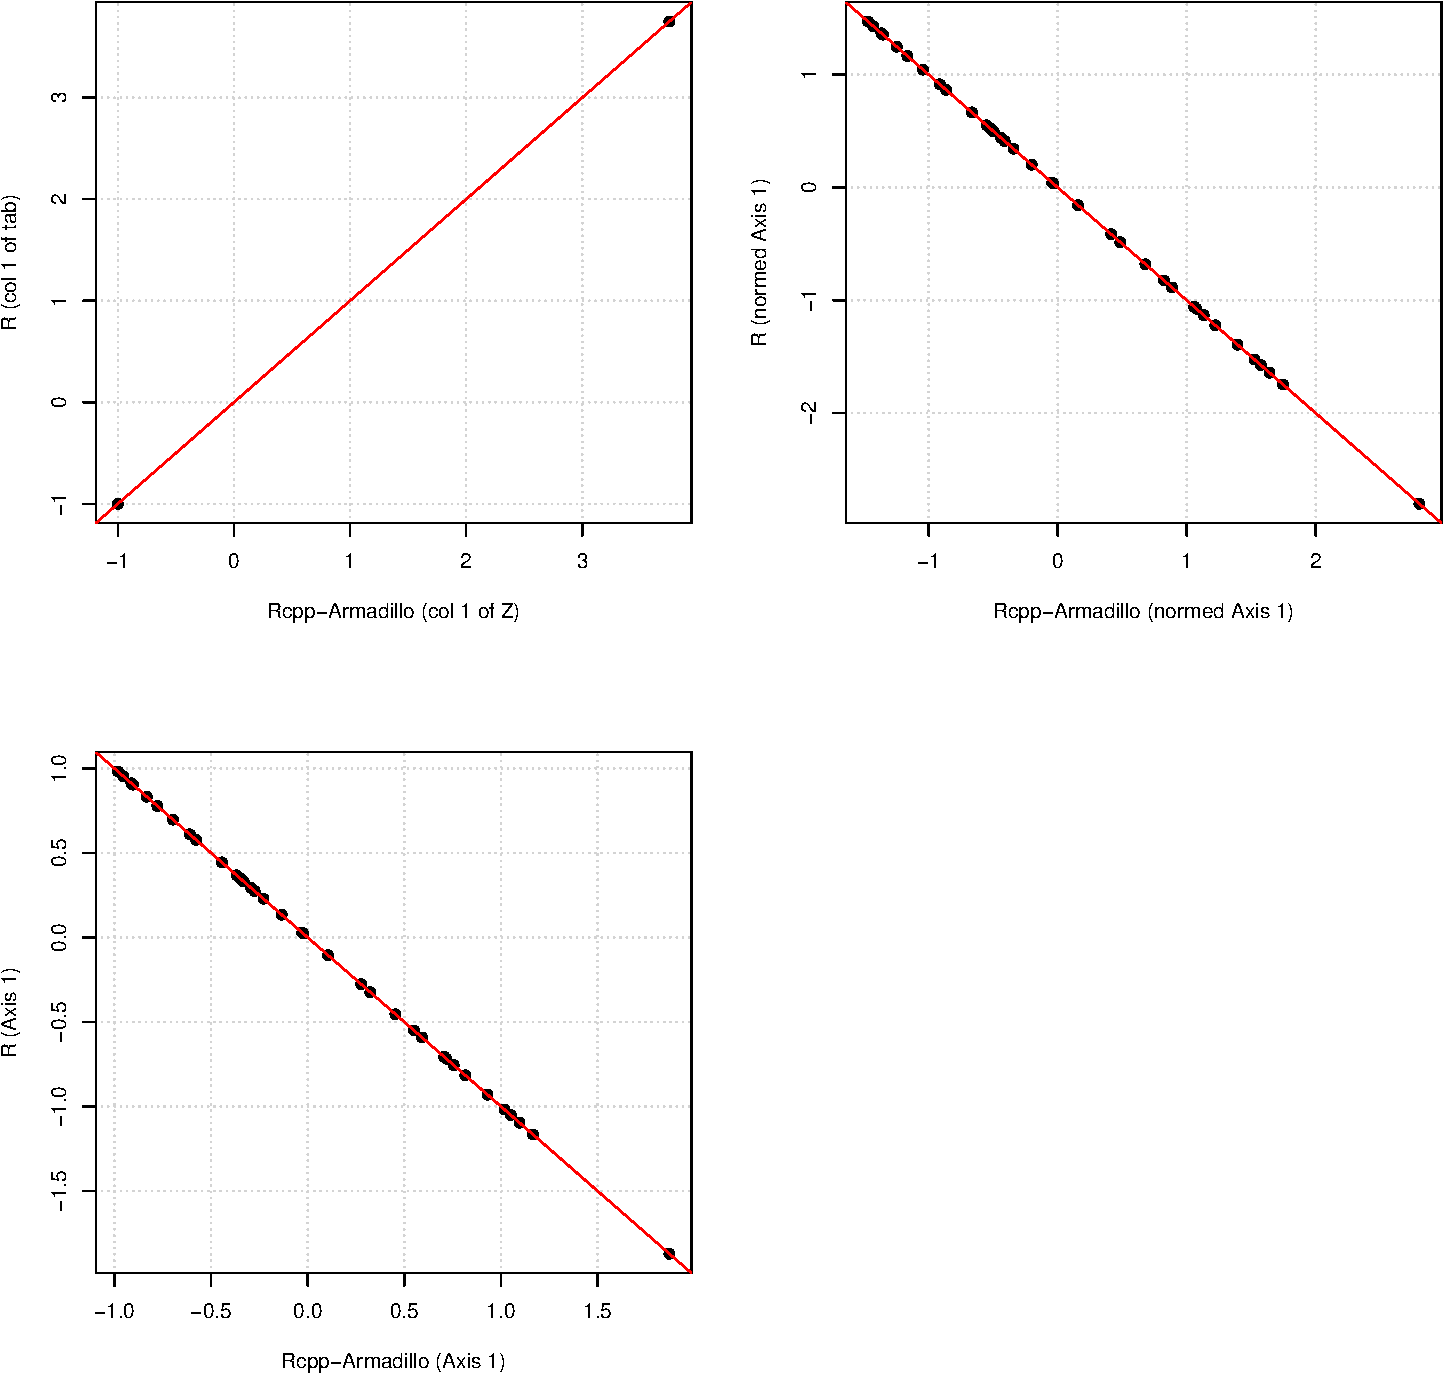
\includegraphics[keepaspectratio]{RandPytonAnalysisPDF_files/RandPytonAnalysisPDF_files/figure-latex/unnamed-chunk-70-1.pdf}}

\section{Multifactorial analysis based on GPU computation with
R}\label{multifactorial-analysis-based-on-gpu-computation-with-r}

see
\url{https://jaredlander.com/content/2021/09/GPUComputingWithR.html\#35}

R packages \textbf{GPUmatrix} and \textbf{torch}

\begin{Shaded}
\begin{Highlighting}[]
\NormalTok{library(GPUmatrix)}
\end{Highlighting}
\end{Shaded}

\begin{verbatim}
## Registered S3 method overwritten by 'bit64':
##   method          from 
##   print.bitstring tools
\end{verbatim}

\begin{verbatim}
## Warning: ModuleNotFoundError: No module named 'tensorflow'
## Run `reticulate::py_last_error()` for details.
## Restart the R session and load the tensorflow R package before reticulate has initialized Python, or ensure reticulate initialized a Python installation where the tensorflow module is installed.
\end{verbatim}

\begin{verbatim}
## Torch tensors allowed
\end{verbatim}

\begin{verbatim}
## Tensorflow tensors allowed
\end{verbatim}

\begin{verbatim}
## Your Torch installation does not have CUDA tensors available. Please check the Torch requirements and installation if you want to use CUDA tensors.
\end{verbatim}

\begin{Shaded}
\begin{Highlighting}[]
\NormalTok{library(torch)}
\end{Highlighting}
\end{Shaded}

\begin{verbatim}
## 
## Attachement du package : 'torch'
\end{verbatim}

\begin{verbatim}
## L'objet suivant est masqué depuis 'package:reticulate':
## 
##     as_iterator
\end{verbatim}

\begin{Shaded}
\begin{Highlighting}[]
\NormalTok{library(ade4)}

\NormalTok{as.dudi.gpu \textless{}{-} function (df, col.w, row.w, scannf, nf, call, type, tol = 1e{-}07, }
\NormalTok{    full = FALSE)\{}
\NormalTok{    if (!is.data.frame(df)) }
\NormalTok{        stop("data.frame expected")}
\NormalTok{    lig \textless{}{-} nrow(df)}
\NormalTok{    col \textless{}{-} ncol(df)}
\NormalTok{    if (length(col.w) != col) }
\NormalTok{        stop("Non convenient col weights")}
\NormalTok{    if (length(row.w) != lig) }
\NormalTok{        stop("Non convenient row weights")}
\NormalTok{    if (any(col.w \textless{} 0)) }
\NormalTok{        stop("col weight \textless{} 0")}
\NormalTok{    if (any(row.w \textless{} 0)) }
\NormalTok{        stop("row weight \textless{} 0")}
\NormalTok{    if (full) }
\NormalTok{        scannf \textless{}{-} FALSE}
\NormalTok{    transpose \textless{}{-} FALSE}
\NormalTok{    if (lig \textless{} col) }
\NormalTok{        transpose \textless{}{-} TRUE}
\NormalTok{    res \textless{}{-} list(tab = df, cw = col.w, lw = row.w)}
\NormalTok{    df \textless{}{-} as.matrix(df)}
\NormalTok{    df.ori \textless{}{-} df}
\NormalTok{    df \textless{}{-} df * sqrt(row.w)}
\NormalTok{    df \textless{}{-} sweep(df, 2, sqrt(col.w), "*")}
\NormalTok{\#\#\#\# conversion matrix into gpu.matrix}
\NormalTok{    df \textless{}{-} as.gpu.matrix(df)}
\NormalTok{    if (!transpose) \{}
\NormalTok{        df \textless{}{-} crossprod(df, df)}
\NormalTok{    \}}
\NormalTok{    else \{}
\NormalTok{        df \textless{}{-} tcrossprod(df, df)}
\NormalTok{    \}}
\NormalTok{    eig0 \textless{}{-} eigen(df, symmetric = TRUE)}
\NormalTok{    eig1 \textless{}{-} list(values = as.vector(Re(eig0$values)),}
\NormalTok{                vectors=as.matrix(Re(eig0$vectors)))}
\NormalTok{    eig \textless{}{-} eig1$values}
\NormalTok{    rank \textless{}{-} sum((eig/eig[1]) \textgreater{} tol)}
\NormalTok{\#\#\# end of GPU computation}
\NormalTok{    if (scannf) \{}
\NormalTok{        if (exists("ade4TkGUIFlag")) \{}
\NormalTok{            nf \textless{}{-} ade4TkGUI::chooseaxes(eig, rank)}
\NormalTok{        \}}
\NormalTok{        else \{}
\NormalTok{            barplot(eig[1:rank])}
\NormalTok{            cat("Select the number of axes: ")}
\NormalTok{            nf \textless{}{-} as.integer(readLines(n = 1))}
\NormalTok{            messageScannf(call, nf)}
\NormalTok{        \}}
\NormalTok{    \}}
\NormalTok{    if (nf \textless{}= 0) }
\NormalTok{        nf \textless{}{-} 2}
\NormalTok{    if (nf \textgreater{} rank) }
\NormalTok{        nf \textless{}{-} rank}
\NormalTok{    if (full) }
\NormalTok{        nf \textless{}{-} rank}
\NormalTok{    res$eig \textless{}{-} eig[1:rank]}
\NormalTok{    res$rank \textless{}{-} rank}
\NormalTok{    res$nf \textless{}{-} nf}
\NormalTok{    col.w[which(col.w == 0)] \textless{}{-} 1}
\NormalTok{    row.w[which(row.w == 0)] \textless{}{-} 1}
\NormalTok{    dval \textless{}{-} sqrt(res$eig)[1:nf]}
\NormalTok{    if (!transpose) \{}
\NormalTok{        col.w \textless{}{-} 1/sqrt(col.w)}
\NormalTok{        auxi \textless{}{-} eig1$vectors[, 1:nf] * col.w}
\NormalTok{        auxi2 \textless{}{-} sweep(df.ori, 2, res$cw, "*")}
\NormalTok{        auxi2 \textless{}{-} data.frame(auxi2 \%*\% auxi)}
\NormalTok{        auxi \textless{}{-} data.frame(auxi)}
\NormalTok{        names(auxi) \textless{}{-} paste("CS", (1:nf), sep = "")}
\NormalTok{        row.names(auxi) \textless{}{-} make.unique(names(res$tab))}
\NormalTok{        res$c1 \textless{}{-} auxi}
\NormalTok{        names(auxi2) \textless{}{-} paste("Axis", (1:nf), sep = "")}
\NormalTok{        row.names(auxi2) \textless{}{-} row.names(res$tab)}
\NormalTok{        res$li \textless{}{-} auxi2}
\NormalTok{        res$co \textless{}{-} sweep(res$c1, 2, dval, "*")}
\NormalTok{        names(res$co) \textless{}{-} paste("Comp", (1:nf), sep = "")}
\NormalTok{        res$l1 \textless{}{-} sweep(res$li, 2, dval, "/")}
\NormalTok{        names(res$l1) \textless{}{-} paste("RS", (1:nf), sep = "")}
\NormalTok{    \}}
\NormalTok{    else \{}
\NormalTok{        row.w \textless{}{-} 1/sqrt(row.w)}
\NormalTok{        auxi \textless{}{-} eig1$vectors[, 1:nf] * row.w}
\NormalTok{        auxi2 \textless{}{-} t(sweep(df.ori, 1, res$lw, "*"))}
\NormalTok{        auxi2 \textless{}{-} data.frame(auxi2 \%*\% auxi)}
\NormalTok{        auxi \textless{}{-} data.frame(auxi)}
\NormalTok{        names(auxi) \textless{}{-} paste("RS", (1:nf), sep = "")}
\NormalTok{        row.names(auxi) \textless{}{-} row.names(res$tab)}
\NormalTok{        res$l1 \textless{}{-} auxi}
\NormalTok{        names(auxi2) \textless{}{-} paste("Comp", (1:nf), sep = "")}
\NormalTok{        row.names(auxi2) \textless{}{-} make.unique(names(res$tab))}
\NormalTok{        res$co \textless{}{-} auxi2}
\NormalTok{        res$li \textless{}{-} sweep(res$l1, 2, dval, "*")}
\NormalTok{        names(res$li) \textless{}{-} paste("Axis", (1:nf), sep = "")}
\NormalTok{        res$c1 \textless{}{-} sweep(res$co, 2, dval, "/")}
\NormalTok{        names(res$c1) \textless{}{-} paste("CS", (1:nf), sep = "")}
\NormalTok{    \}}
\NormalTok{    res$call \textless{}{-} call}
\NormalTok{    class(res) \textless{}{-} c(type, "dudi")}
\NormalTok{    return(res)}
\NormalTok{\}}

\NormalTok{dudi.pca.gpu \textless{}{-} function (df, row.w = rep(1, nrow(df))/nrow(df), col.w = rep(1, }
\NormalTok{    ncol(df)), center = TRUE, scale = TRUE, scannf = TRUE, nf = 2)\{}
\NormalTok{    df \textless{}{-} as.data.frame(df)}
\NormalTok{    nc \textless{}{-} ncol(df)}
\NormalTok{    if (any(is.na(df))) }
\NormalTok{        stop("na entries in table")}
\NormalTok{    f1 \textless{}{-} function(v) sum(v * row.w)/sum(row.w)}
\NormalTok{    f2 \textless{}{-} function(v) sqrt(sum(v * v * row.w)/sum(row.w))}
\NormalTok{    if (is.logical(center)) \{}
\NormalTok{        if (center) \{}
\NormalTok{            center \textless{}{-} apply(df, 2, f1)}
\NormalTok{            df \textless{}{-} sweep(df, 2, center)}
\NormalTok{        \}}
\NormalTok{        else center \textless{}{-} rep(0, nc)}
\NormalTok{    \}}
\NormalTok{    else if (is.numeric(center) \&\& (length(center) == nc)) }
\NormalTok{        df \textless{}{-} sweep(df, 2, center)}
\NormalTok{    else stop("Non convenient selection for center")}
\NormalTok{    if (scale) \{}
\NormalTok{        norm \textless{}{-} apply(df, 2, f2)}
\NormalTok{        norm[norm \textless{} 1e{-}08] \textless{}{-} 1}
\NormalTok{        df \textless{}{-} sweep(df, 2, norm, "/")}
\NormalTok{    \}}
\NormalTok{    else norm \textless{}{-} rep(1, nc)}
\NormalTok{    X \textless{}{-} as.dudi.gpu(df, col.w, row.w, scannf = scannf, nf = nf, }
\NormalTok{        call = match.call(), type = "pca")}
\NormalTok{    X$cent \textless{}{-} center}
\NormalTok{    X$norm \textless{}{-} norm}
\NormalTok{    X}
\NormalTok{\}}


\NormalTok{\#\#\#\# test}
\NormalTok{data(deug)}
\NormalTok{dudi1 \textless{}{-} dudi.pca(deug$tab, center = TRUE, scale = TRUE, scan = FALSE)}
\NormalTok{dudi2 \textless{}{-} dudi.pca.gpu(deug$tab, center = TRUE, scale = TRUE, scan = FALSE)}
\end{Highlighting}
\end{Shaded}

test with linear algebric functions from the R package \textbf{torch}:

\begin{Shaded}
\begin{Highlighting}[]
\NormalTok{library(torch)}
\NormalTok{apropos("linalg")}
\NormalTok{\#  [1] "linalg\_cholesky"            "linalg\_cholesky\_ex"         "linalg\_cond"                "linalg\_det"                }
\NormalTok{\#  [5] "linalg\_eig"                 "linalg\_eigh"                "linalg\_eigvals"             "linalg\_eigvalsh"           }
\NormalTok{\#  [9] "linalg\_householder\_product" "linalg\_inv"                 "linalg\_inv\_ex"              "linalg\_lstsq"              }
\NormalTok{\# [13] "linalg\_matrix\_norm"         "linalg\_matrix\_power"        "linalg\_matrix\_rank"         "linalg\_multi\_dot"          }
\NormalTok{\# [17] "linalg\_norm"                "linalg\_pinv"                "linalg\_qr"                  "linalg\_slogdet"            }
\NormalTok{\# [21] "linalg\_solve"               "linalg\_svd"                 "linalg\_svdvals"             "linalg\_tensorinv"          }
\NormalTok{\# [25] "linalg\_tensorsolve"         "linalg\_vector\_norm"  }
\end{Highlighting}
\end{Shaded}

\section{Multifactorial analysis based on GPU computation with
Python}\label{multifactorial-analysis-based-on-gpu-computation-with-python}

In this section, the library \textbf{cupy} (\url{https://cupy.dev/}) is
used to implement the duality diagram.

\begin{Shaded}
\begin{Highlighting}[]
\NormalTok{import os}
\NormalTok{import string}
\NormalTok{import re}
\NormalTok{import pandas as pd}
\NormalTok{import numpy as np}
\NormalTok{import cupy as cu}

\NormalTok{def cupydudi(X,cw,lw,nf):}
\NormalTok{  dim = X.shape}
\NormalTok{  n = dim[0]}
\NormalTok{  p = dim[1]}
\NormalTok{  nf0 = nf{-}1}
\NormalTok{  \# n=len(X)}
\NormalTok{  \# p=len(X.columns)}
\NormalTok{  D = cu.diag(cu.sqrt(lw))}
\NormalTok{  Q = cu.diag(cu.sqrt(cw))}
  
\NormalTok{  \# XtDXQ =\textgreater{} problem  with Q !!!}
  
\NormalTok{  XD = cu.dot(X.T,D).T}
\NormalTok{  XD = cu.dot(XD,Q)}
\NormalTok{  XtX = cu.dot(XD.T,XD)}
  
  
\NormalTok{  \# decomposition}
\NormalTok{  eigenvalues, eigenvectors = cu.linalg.eig(XtX)}
\NormalTok{  index = cu.argsort(eigenvalues)[::{-}1]}
  
\NormalTok{  \# np.nonzero(eigenvalues)[0]}
\NormalTok{  eigenvalues = eigenvalues.real}
\NormalTok{  eigenvectors = eigenvectors.real}
\NormalTok{  eigenvalues=eigenvalues[index]}
\NormalTok{  eigenvectors=eigenvectors[:,index]}
\NormalTok{  \# results}
\NormalTok{  rank = len(cu.nonzero(eigenvalues)[0])}
\NormalTok{  C1 = cu.dot(cu.diag(1/cu.sqrt(cw)),eigenvectors[:,0:nf])}
\NormalTok{  \#C1 = eigenvectors[:,0:nf]}
\NormalTok{  XQ = cu.dot(X,cu.diag(cw))}
\NormalTok{  Li = cu.dot(XQ, C1)}
  
\NormalTok{  \# need to adjust the weighting (problem with sqrt)}
\NormalTok{  L1 = cu.dot(Li,cu.diag(1/cu.sqrt(eigenvalues[0:nf])))}
\NormalTok{  Co = cu.dot(C1,cu.diag(cu.sqrt(eigenvalues[0:nf])))}
\NormalTok{  return eigenvalues,rank,Li,L1,Co,C1,nf;}

\NormalTok{\#\#\#}
\end{Highlighting}
\end{Shaded}

\section{Future development for the Package
pydudi}\label{future-development-for-the-package-pydudi}

modification of the names used for the function (?)

\begin{itemize}
\tightlist
\item
  check names and use of the function
\item
  add acmutil function for the preparation of the Burt's table
\end{itemize}

implementation in python:

\begin{itemize}
\tightlist
\item
  class Ktab
\item
  function coinertia
\item
  function pls
\item
  function spls
\item
  function gpls
\item
  function mbpls
\item
  function smbpls
\item
  function statis
\item
  function mfa
\item
  function mcoa
\item
  function gpa
\item
  function coinertia
\end{itemize}

NOTA: The objective of this works is not to replace the R package ade4,
but it's just a manner to improve my skill in python.

\section{References}\label{references}

\begin{itemize}
\tightlist
\item
  R \url{http://www.R-project.org/}.
\item
  R Core Team (2013). R: A language and environment for statistical
  computing. R Foundation for Statistical Computing, Vienna, Austria.
  URL \url{http://www.R-project.org/}.
\item
  Dray S, Dufour A (2007). ``The ade4 Package: Implementing the Duality
  Diagram for Ecologists.'' \emph{Journal of Statistical Software},
  \emph{22}(4), 1-20. \url{doi:10.18637/jss.v022.i04}
  \url{https://doi.org/10.18637/jss.v022.i04}.
\item
  Chessel D, Dufour A, Thioulouse J (2004). ``The ade4 Package - I:
  One-Table Methods.'' \emph{R News}, \emph{4}(1), 5-10.
  \url{https://cran.r-project.org/doc/Rnews/}.
\item
  Dray S, Dufour A, Chessel D (2007). ``The ade4 Package - II: Two-Table
  and K-Table Methods.'' \emph{R News}, \emph{7}(2), 47-52.
  \url{https://cran.r-project.org/doc/Rnews/}.
\item
  Thioulouse J, Dray S, Dufour A, Siberchicot A, Jombart T, Pavoine S
  (2018). \emph{Multivariate Analysis of Ecological Data with ade4}.
  Springer. \url{doi:10.1007/978-1-4939-8850-1}
  \url{https://doi.org/10.1007/978-1-4939-8850-1}.
\item
  Escoufier, Y. (1987) The duality diagram : a means of better practical
  applications In Development in numerical ecology, Legendre, P. \&
  Legendre, L. (Eds.) NATO advanced Institute, Serie G. Springer Verlag,
  Berlin, 139--156.
\item
  Benzécri, J.P. and Coll. (1973) \emph{L'analyse des données. II
  L'analyse des correspondances}, Bordas, Paris. 1-620.
\item
  Greenacre, M. J. (1984) \emph{Theory and applications of
  correspondence analysis}, Academic Press, London.
\item
  Tenenhaus, M. \& Young, F.W. (1985) An analysis and synthesis of
  multiple correspondence analysis, optimal scaling, dual scaling,
  homogeneity analysis ans other methods for quantifying categorical
  multivariate data. Psychometrika, 50, 1, 91-119.
\item
  Lebart, L., A. Morineau, and M. Piron. 1995. Statistique exploratoire
  multidimensionnelle. Dunod, Paris.
\end{itemize}

\section{Appendix}\label{appendix}

\subsection{Additional R functions}\label{additional-r-functions}

zzz

\subsection{Session information}\label{session-information}

\begin{Shaded}
\begin{Highlighting}[]
\NormalTok{print(sessionInfo(),locale=FALSE)}
\end{Highlighting}
\end{Shaded}

\begin{verbatim}
## R version 4.6.0 (2026-04-24)
## Platform: x86_64-pc-linux-gnu
## Running under: Linux Mint 21.3
## 
## Matrix products: default
## BLAS:   /usr/lib/x86_64-linux-gnu/blas/libblas.so.3.10.0 
## LAPACK: /usr/lib/x86_64-linux-gnu/lapack/liblapack.so.3.10.0  LAPACK version 3.10.0
## 
## attached base packages:
## [1] parallel  graphics  datasets  utils     stats     tools     grDevices methods  
## [9] base     
## 
## other attached packages:
##  [1] torch_0.15.0           GPUmatrix_1.0.2        RcppArmadillo_14.6.0-1
##  [4] Rcpp_1.1.1-1.1         reticulate_1.46.0      circlize_0.4.16       
##  [7] xtable_1.8-4           tinytex_0.57           rmarkdown_2.31        
## [10] knitr_1.51             pixmap_0.4-13          ade4_1.7-23           
## [13] RColorBrewer_1.1-3    
## 
## loaded via a namespace (and not attached):
##  [1] Matrix_1.7-5        bit_4.6.0           jsonlite_2.0.0      compiler_4.6.0     
##  [5] tensorflow_2.16.0   callr_3.7.6         tfruns_1.5.3        png_0.1-8          
##  [9] yaml_2.3.10         fastmap_1.2.0       lattice_0.22-7      here_1.0.1         
## [13] shape_1.4.6.1       MASS_7.3-65         rprojroot_2.0.4     pillar_1.11.0      
## [17] rlang_1.3.0         xfun_0.52           GlobalOptions_0.1.2 bit64_4.6.0-1      
## [21] otel_0.2.0          cli_3.6.5           magrittr_2.0.5      withr_3.0.2        
## [25] ps_1.9.1            processx_3.8.6      digest_0.6.37       grid_4.6.0         
## [29] rstudioapi_0.17.1   base64enc_0.1-6     lifecycle_1.0.5     vctrs_0.7.3        
## [33] coro_1.1.0          glue_1.8.0          evaluate_1.0.4      whisker_0.4.1      
## [37] colorspace_2.1-1    htmltools_0.5.9
\end{verbatim}

\end{document}
